
\documentclass[10pt,letterpaper, notitlepage]{article}
\usepackage[utf8]{inputenc}
\usepackage[T1]{fontenc}
\usepackage{amsmath}
\usepackage{amsfonts}
\usepackage{amssymb}
\usepackage{graphicx}
\usepackage[noabbrev]{cleveref}
\usepackage{mathrsfs}
\usepackage{mathtools}
\usepackage{enumerate}
\usepackage[margin=1in]{geometry}
\usepackage{color}
\usepackage{authblk}
\usepackage{booktabs}
\usepackage{longtable}
\usepackage{array}
\usepackage{multirow}
\usepackage{wrapfig}
\usepackage{float}
\usepackage{colortbl}
\usepackage{pdflscape}
\usepackage{tabu}
\usepackage{threeparttable}
\usepackage{threeparttablex}
\usepackage[normalem]{ulem}
\usepackage{makecell}
\usepackage{xcolor}

\usepackage{todonotes}

%%
\linespread{1.5}
\newcommand{\Normal}{\operatorname{Normal}}
\newcommand{\Gmma}{\operatorname{Gamma}}
\newcommand{\Lognormal}{\operatorname{Lognormal}}

%Import the natbib package and sets a bibliography  and citation styles
\usepackage[round, sort, numbers]{natbib}
\setcitestyle{square}
\bibliographystyle{unsrtnat}
%%

\title{Developing and Evaluating Pharmacokinetics-Driven \\Dynamic Personalized Medicine: A Framework and Case Study}

%\author{A. Demetri Pananos M.Math, Rommel G. Tirona Ph.D, Simon Bonner Ph.D,  Daniel J. Lizotte Ph.D}
\author[1, *]{A. Demetri Pananos, M.Math}
\author[2]{Rommel G. Tirona Ph.D}
\author[3]{Simon Bonner Ph.D}
\author[1,4]{Daniel J, Lizotte, Ph.D}
\affil[1]{Department of Epidemiology and Biostatsitics, Western University}
\affil[2]{Department of Physiology and Pharmacology, Western University}
\affil[3]{Department of Statistics and Actuarial Sciences, Western University}
\affil[4]{Department of Computer Science, Western University}
\affil[*]{Corresponding Author}

\setcounter{Maxaffil}{0}
\date{}


\begin{document}
	\begin{titlepage}
	\maketitle
	
	Word count: 4496
	\footnote{Financial support for this study was provided by Ontario Research Fund and Natural Sciences and Engineering Research Council of Canada. The funding agreement ensured the authors’ independence in designing the study, interpreting the data, writing, and publishing the report.}
	\end{titlepage}

	
	% Second title page
	\begin{titlepage}
		\centering
		\vskip 60pt
		\topskip0pt
		\vspace*{\fill}
		\LARGE Developing and Evaluating Pharmacokinetics-Driven \\Dynamic Personalized Medicine: A Framework and Case Study \par
		\vskip 3em
		\vspace*{\fill}
		\large %Author A, Author B \par
		%\vskip 1.5em
		Acknowledgements: The authors wish to thank A.J.B for their comments on health economic impacts of this work, as well as R.K and their lab for providing pharmacological expertise.
	\end{titlepage}

\begin{abstract}
\textbf{Background}: One goal of personalized medicine is to select the right dose for a drug by considering factors which may explain variability in effectiveness or toxicity. Most efforts to personalize dose size seek to inform dose selection at a single time, with the goal of eliminating the need for dose adjustments (titration). We refer to this as static personalization. Despite progress, the need for titration has not been eliminated and thus there is an opportunity to personalize the titration process as well. We refer to this as dynamic personalization. Despite its potential to improve care, dynamic personalization imposes additional burden on the patient and provider, because it requires ongoing monitoring, for example by gathering lab results and requiring additional clinic visits. It is natural to ask:  is the additional control over dose worth the additional burden?
\textbf{Objective}: To develop a framework for the simulation based evaluation of static and dynamic personalization based on pharmacokinetic modelling.Methods: We frame dynamic personalization as a dynamic treatment regime and describe how Bayesian pharmacokinetic models can be used to estimate the optimal policy with Q learning, and we propose a simulation-based strategy for internal evaluation.
 \textbf{Results}: We demonstrate the use of our framework to investigate the potential benefits of static and dynamic personalization for apixaban dosing.
 \textbf{Conclusions}: The proposed framework can help compare potential burden and benefits of different modes of personalized dosing and it can be integrated with other system level decision making frameworks in order to evaluate whether such a personalized medicine program should be implemented into a particular health care system.


\end{abstract}

	\section{Introduction}

Personalized medicine has four goals: 1) to identify drugs for which between-subject variability in effectiveness or toxicity is a key issue for effective treatment, 2) to identify predictors which may explain this variability, 3) to decide on the right dose of the right drug by considering these factors, and 4) prevent adverse reactions to drugs \cite{morse2015personalized}.  Progress in all four goals has accelerated within the last decade. As an example, recent studies on DPYD genotype testing prior to starting fluoropyrimidine-based chemotherapy showed promise in preventing adverse events, making good arguments for integration of DPYD genotype testing into standard of care practices \cite{wigle2019prospective}. Despite this progress, personalized medicine still faces several barriers to widespread adoption, including economic burden, patient burden, and expertise burden required for new methods of personalization.


Personalized medicine reduces costs to the healthcare system by identifying patients who are at greater risk for adverse events or dose adjustments, thereby optimizing safety.  If the patient does not undergo an adverse event, then this ultimately saves the healthcare system the cost of the hospital stay \cite{looff2016economic}.  More ambitiously, personalized medicine has the potential to save the healthcare system costs by more effectively using resources \cite{shabaruddin2015economic}. The cost of instruments, technicians, and leadership required to operate a personalized medicine clinic are high burden, and it is not yet clear if personalized medicine is sufficiently cost effective to offset operating costs in all circumstances \cite{kasztura2019cost}.  In their 2019 scoping review of personalized medicine cost effectiveness, Kasztura et. al \cite{kasztura2019cost} found that willingness-to-pay thresholds vary wildy from country to country (citing that cost per quality adjusted life year for some modes of personalized medicine range from \$20, 000 USD per quality adjusted life year in for studies in Europe and the United Kingdom to \$200,000 USD per quality adjusted life year for studies in the United States).  This high variability in cost effectiveness means the burden required for start up may result in a positive return on investment in some areas but not others. This variability should prompt would be adopters to more closely examine if taking on the initial burden is worth the result.


% beef up here
% Examples.  Identifty clear examples from the literature around diagnostics?
The dominant perspective on personalized medicine focuses on the use of clinical and physioligical information (including biomarkers, genotyping, and diagnostic tests) as a means of optimizing treatments, but largely ignore needs, constraints, and utilities of the patient \cite{rogowski2015concepts, di2017personalized}. Patients can be burdened by frequent followup for clinical measurement (as in the case with Warfarin), be burdended by costly expenses related to obtaining care, or may be more risk adverse/tolerant than the ``typical'' patient. As an example, transportation has been found to be a large financial burden for patients recieving cancer treatment \cite{houts1984nonmedical}, and continues to burden patients, with a 2020 study finding that the cost of parking alone can climb as high as \$1600 over the course of treatment in the United States \cite{lee2020assessment}.  Additional visits to a clinic have the potential to further burden patients by requiring them to miss a day of work, and find means of childcare during their absence (if neccesary). Incorporating patient preferences and reducing the burden of personalization on the patient can result in sustained adherence \cite{elliott2008understanding}, thereby increasing effectiveness and further preventing adverse events.


% FInd some machine learning cautinary tales

An additional expertise burden is added as machine learning (used interchangeably with the term “artificial intelligence”) is adopted into personalized medicine initiatives.  Cutting edge machine learning models for prediction or decision making can be prohibitively burdensome to implement effectively. Failure to do so may result in pernicious bias inadvertently affecting subpopulations, as was found to be the case in algorithms for credit scoring \cite{barocas2016big}, crime prediction \cite{lum2016predict}, and hiring \cite{ajunwa2020paradox}.  A 2019 study found an instance of this bias in a widely used risk scoring algorithm in healthcare \cite{obermeyer2019dissecting}, demonstrating that despite the best intentions of those involved, the use of a model can lead to worse rather than better care if investigators are not careful in considering what sorts of bias may be present in the data used to train these models.  Implementation of new approaches and methods requires the close collaboration of experts in data science  with physicians, domain experts, and other stakeholders.  Close collaboration should allow for domain experts to identify what kinds of biases the data might have, and for data science experts to implement methods to help ammeliorate that bias (or to admit the data are not fit for purpose).  The result of iterating on this collaborative process (wherein domain experts help inform the appraoches methodologists take, and the methodologists provide model checks which help domain experts decide if decisions from the model are reasonable or suspicious) is a model which more closely aligns with domain expertise, a model which is sufficiently flexible to capture the true data generating mechanism, an effective use of data, a more transparent modelling process, and calibrated expectations surrounding algorithms and their abilities \cite{frohlich2018hype}.  Presently, this form of collaboration between methodologists and domain experts is not the norm, with developement of machine learning solutions in healthcare bdeing developed in silos \cite{wiens2019no}.

These burdens may be surmountable for some, but the question then turns to if the result is worth the expense.  Answering that question is difficult without an idea how the additional burden of collecting data, or implementing new algorithms, will benefit the clinic or the patient subject to inherent constraints. 

 In this study, we present a new framework for helping practitioners interested in implementing personalized medicine to answer a) If the burden of personalization could result in more favorable outcomes for their population of patients, b) how working around patient burden (such as coming into the clinic for fewer measurements) may change effectiveness, and c) if more complex models for personalization can lead to better effectiveness. For our case study, we fit a Bayesian model to existing data on the pharmacokinetics of apixaban.  The resulting Bayesian model is used to generate synthetic pharmacokinetic data for use in experiments to compare different forms of personalization. Treating personalization as a dynamic treatment regime, we propose six policies, each increasing in complexity and clinic/patient burden, for personalizing doses of apixaban with the goal of keeping blood serum concentrations within a desired range for as long as possible. Under the assumption that the fitted Bayesian model can produce similar data to what might be observed in the future from new patients, we can make inferences as to how different policies for personalizing doses may improve upon one another, and compare if the additional burden of implementing a more complex or costly form of personalization can generate a more desirable outcome for the patient or healthcare provider.  

We begin with an overview of dynamic treatment regimes.  We then describe how to estimate an optimal dynamic treatment regime  by combining Bayesian pharmacokinetic modelling with Q-learning.  We then present our case study, beginning with the details of the Bayesian model we use to fit the real pharmacokinetic data, and present model fit diagnostics to argue that our model is satisfactory for generating synthetic data for use in our simulations. We then present and discuss the results of our simulation in light of the burden presented to a clinic to implement personalized medicine, and how this framework can be integrated to answer questions such as if personalization can produce a positive return on investment, how burdening the patient with an additional clinic visit will improve the clinic's understanding of how to treat that patient, and if using a more advanced mode of personalization will result in more favortable health outcomes.
%Given these three types of burden, want to assess if it is worth doing or not.
% Concrete examples from the three burdens 

	\section{Background}\label{ss:background}

In the following two subsections, we present background material on dynamic treatment regimes, which are used to develop optimal decision-making models, and Bayesian PK models, which are used to capture relationships among patient characteristics, measurements, pharmacokinetics, and dose so that optimal dosing decisions can be derived using the dynamic treatment regime framework.

\subsection{Dynamic Treatment Regimes}

In this section, we review the theory of dynamic treatment regimes and how dynamic personalization using PK models can be formulated using a dynamic treatment regime.

Our work considers personalization of a dose or sequences of doses for a patient with the aim of keeping their blood serum concentration of a drug within a desired range for as long as possible given two practical constraints: first we are limited to baseline measurements of clinical variables (e.g., age, weight) to make our initial dosing decision, and second the subject’s blood concentration cannot be measured very frequently after the initial dose. The theory of dynamic treatment regimes and statistical reinforcement learning offers a way of operationalizing optimal dynamic personalization that combines baseline information with subsequent blood concentration information to select initial and subsequent doses that optimize a chosen criterion, like for example time spent in therapeutic range.

A dynamic treatment regime (DTR) is a sequence of decision rules for adapting a treatment plan to the time-varying state of an individual subject \cite{chakraborty2013statistical}. In DTRs, and their cousin topic in computer science \textit{reinforcement learning}, an agent (often thought of as a robot in reinforcement learning, but within medicine sometimes thought of as a physician’s computerized decision support system) interacts with a system for a number of stages. At each stage, the agent receives an \textit{observation} of the system and then decides which \textit{action} to take.  This action will result in an observed \textit{reward} which is followed by a new observation of the system after it has been impacted by the action.  This cycle of observation, action, reward then repeats, with the agent aiming to take actions which yield the largest total reward.

\subsubsection{Trajectories}

The data generated by the cycle of observation, action, and reward from the inial action to the final reward is called a \textit{trajectory}. Formally, we define a stage to be a triple containing an observation, chosen action, and resulting reward. Let $O_i$ denote an observation at the $i^{th}$ stage, $ A_i $ be the action at the $ i^{th} $ stage, and $ Y_i $ denote the reward at the $ i^{th}$ stage, denoted in capital letters when considering the observation, action, and reward as random variables.  A  trajectory is then the tuple $ (O_1, A_1, O_2, A_2,  \cdots, O_K, A_K, O_{K+1})$.  Following notation by Chakraborty and Moodie \cite{chakraborty2013statistical}, we will denote a system’s history at stage $ j $ as $ H_j = (O_1, A_1, O_2, A_2, \cdots , O_{j-1}, A_{j-1}, O_j) $.  The reward at stage $j$ is then a function of the system’s history, the action taken, and the next observation $ Y_j = Y_j(H_j, A_j, O_{j+1}) $.

\subsubsection{Policies, Value Functions, and Q-Learning}

A policy $ d = (d_1, \cdots, d_k) $ is a vector of decision rules each of which take as input the system’s history and output an action to take.  Each decision rule is a function $d_j : \mathcal{H}_j \to \mathcal{A}_j$ where $\mathcal{H}_j$ and $\mathcal{A}_j$ are the history and action spaces at stage $j$ respectively.  The stage $ j $ value function for a policy $ d $ is the expected reward the agent would receive starting from history $ h_j  $(here in lower case since it is an observed quantity) if it chose actions according to $ d $ for every action thereafter.  The value function is written as
\begin{equation}
	V^d_j(h_j) = E_d\left[ \sum_{k=j}^K Y_k(H_k, A_k, O_{k+1}) \Bigg\lvert H_j = h_j\right] \>.
\end{equation}

\noindent Here, the expectation is over the distribution of trajectories. Importantly, the stage $ j $ 
value function can be decomposed into the expectation of reward at stage $ j $ plus the stage $ j+1  $ value function  \cite{chakraborty2013statistical}
\begin{equation}
V^d_j(h_j) = E_d\left[Y_j(H_j, A_j, O_{j+1}) + V^d_{j+1}(H_{j+1}) \vert H_j = h_j\right] \>.
\end{equation}


\noindent The optimal stage $ j  $ value function is the value function under a policy which yields maximal value. 

\begin{equation}
V^{opt}_j(h_j) = \underset{d \in \mathscr{D}}{\mbox{max}} V^d_j(h_j)
\end{equation}

\noindent  Estimating a policy that maximizes value can be achieved by estimating the optimal Q function \cite{chakraborty2013statistical}.  The optimal Q function at stage $ j $ is a function of the system’s history $ h_j $ and a proposed action $ a_j $,
\begin{equation}
 Q_j^{opt} = E \left[ 
 Y_j(H_j, A_j, O_{j+1}) + V^{opt}_{j+1}(H_{j+1}) \lvert H_j = h_j, A_j = a_j
 \right].
\end{equation}

Note that the optimal Q function has similar form and interpretation to the optimal value function (namely, it is the expected reward starting at stage $ j $ but with the added condition that we take action $ a_j $ and then follow the optimal policy thereafter). Due to the decomposition of the reward function at stage $ j $, estimation of the optimal Q function can be performed by choosing the action which yields the largest reward at each stage assuming we act optimally in the future. 

Given the optimal Q function, an optimal policy is given by 
\begin{equation}
d_j^{opt}(h_j,a) = \arg\max_{a} Q_j^{opt}(h_j,a).
\end{equation}
To use Q-learning for personalization in the context of optimal dosing and titration, we will define the actions to be possible doses or dose adjustments, and we define the reward to be a function of the resulting concentrations, for example a measurement of how well concentrations are kept in a specified therapeutic range. The relationship between possible actions and rewards, which Q-learning can use to produce optimal policies, can be captured by Bayesian PK modelling, which we now review.

\subsection{Bayesian Models of Pharmacokinetics}

In order to estimate the optimal Q functions, we need to be able to predict how a patient's concentration is likely to evolve over time in response to a hypothetical dose (action.)  Our approach is to build a Bayesian model of patient pharmacokinetics that can use baseline clinical information, as well as any available concentration measurements, to make tailored predictions of future concentrations that are as accurate as possible given the model structure and available data. The model is flexible in that it can condition on whatever information is available---for example, if previous dose and measurement information is not available for a specific patient, the model will rely on baseline information alone. If it is available, the model will use it to (hopefully) make improved predictions. This allows us to optimize both initial doses and later dose adjustments after additional information about concentration is acquired.

Bayesian models have another key property that we use in our framework. They are able to simulate the trajectories of patients drawn from a distribution that is similar to the distribution of the data that the models were trained on, but in the simulated data, \textit{all} variables---including normally-hidden PK parameters---are fully observed. This allows us to conduct a form of internal validation where we use the simulated patients to assess the relative benefits of different modes of static and dynamic personalization, because we can know for each simulated patient exactly what the effect of any dose would be. This process is described in detail in the next section, where we present our framework, and the details of the Bayesian model itself are provided in Appendix~\ref{ap:appendix}.

	\section{A Framework for Assessing Static and Dynamic Personalization}\label{ss:framework}

In this section, we present the components of our framework for assessing static and dynamic personalization, including details for fitting a hierarchical Bayesian PK model to concentration data from a cohort of patients, assessing the behaviour of Markov chains via diagnostics, and using the Bayesian model to generate simulated data for evaluation. We then outline several modes of static and dynamic personalization ranging from no personalization (every patient gets the same dose) to a complex dynamic mode of personalization (estimation of the optimal policy for dosing from a dynamic treatment regime).  Finally, we outline steps for assessing the benefits of each mode of personalization.

\subsection{Bayesian Modelling}

The first step in our framework is to fit a Bayesian model that relates patient covariates and dose to drug concentration as a function of time. For example, previous work \cite{pananos2020comparisons} describes a hierarchical Bayesian model of apixaban pharmacokinetics, in which the clearance (L/hour), time to maximum concentration (hours), absorption time delay (hours), and ratio between the elimination and absorption rate constants (called alpha, a unitless parameter) are hierarchically modelled. In our case study, we extend that model by regressing the latent pharmacokinetic parameters on baseline clinical variables (age, sex, weight, and creatinine) to permit personalization. The model could equally well be extended with pharmacokinetic or biomarker information if the relevant theory and data were available for a particular use case. See \cref{ap:appendix} for our model details.

Once the form of the model is specified, creating simulated patients or estimating the PK parameters of a real patient requires computation of or sampling from the posterior distribution of the relevant variables given the relevant data. However, exact computation of the posterior distribution is intractable for all but very simple models, so Markov chain Monte Carlo (MCMC) techniques are often used to approximate the expectations with respect to the posterior distribution.  Presently, the gold standard for generating samples from the posterior is Hamiltonian Monte Carlo (HMC), which works by generating a sequence of samples that ``explores'' the posterior distribution by solving a system of ordinary differential equations which describe the motion of an imaginary particle as it rolls along the surface of the log posterior density.  Many implementations of HMC come with diagnostics which monitor the behaviour of the Markov chains that are used to generate samples and help to ensure that they are representative of the posterior distribution. That these Markov chains behave well is crucial, as any inferences about or from the model are obtained from samples generated by the chains. To assess the quality of the Markov chains, several diagnostics are commonly used including: number of divergences, the Gelman-Rubin convergence diagnostic, and effective sample size \cite{betancourt2018conceptual}.

In practice, several Markov chains are used simultaneously to generate samples from the posterior. The chains are assessed with within-chain and between-chain diagnostics. First, individual chains may sometimes \textit{diverge}. A divergence in a Markov chain indicates that the HMC Markov chain has encountered a region of high curvature in the posterior distribution which cannot be adequately explored.  Consequently, Monte Carlo estimators of any expectations can be biased due to incomplete exploration of the posterior distribution.  It is important that none of the Markov chains generated by HMC display a divergence, and that many chains (typically 4 or more) are initialized and are allowed to explore the posterior distribution. 

Having ensured that no chains are diverging, a group-level diagnostic is used to assess whether all chains have converged to the same limiting distribution.  The \textit{Gelman-Rubin (sometimes called $\hat{R}$) convergence diagnostic} is designed to detect if the Markov chains have converged to the same distribution by measuring the within-chain variance to the between chain-variance. In practice, $1.05<\hat{R}$ indicates that there is poor mixing of the Markov chains and inference from the samples should not be performed lest the Monte Carlo estimators are biased by this poor mixing.

Even if the chains do not exhibit divergences and arrive at the same limiting distribution, the Markov chains could still exhibit high within-chain correlation, thereby increasing the uncertainty of estimation of key posterior quantities such as means, variances, or quantiles \cite{brooks2011handbook}.  The \textit{effective sample size} is a measure of how much the within chain autocorrelation increases uncertainty estimates.  In some software packages, the effective sample size is reported as a fraction of the total number of samples drawn from the Markov chains.  Presently, the guidance is that the effective sample size ratio should be no smaller than 1\%.



In addition to monitoring divergences, Gelman-Rubin convergence diagnostics, and effective sample sizes, the model should be evaluated against existing domain knowledge.  Evaluating that the model has learned appropriate  behaviour (e.g. that as one quantity increases, another should decrease) can be performed by plotting model predictions.  Additionally, \textit{posterior predictive checks} -- generating synthetic data  from the model's posterior distribution and comparing against the real data -- can be performed to ensure the model is not generating data which are physically impossible or completely unrealistic. Once the model is fit, important diagnostics indicate no pathalogical behaviour, and the model is deemed to fit the data sufficiently well, the model can then used to generate synthetic pharmacokinetic data for use in experiments to compare different forms of personalization. Each generated data point may be thought of as one synthetic patient, with observed covariates and observed pharmacokinetic parameters. These parameters, which are never observed in real data, allow us to compute the effects of any dosing decisions (which are made \textit{without} direct knowledge of the parameters), and thus allow us to evaluate the performance of different modes of personalized dosing on the sampled population. 

\subsection{Modes of Personalization \& Assessment of Personalization}

The second step in our framework is to identify modes of personalization that we wish to evaluate. We classify these modes of personalization into two types: static and dynamic personalization.

Static modes of personalization seek to inform the dose at one point in time (usually treatment initiation) with the goal of eliminating the need for ``trial-and-error'' adjustments.  We consider two modes of static personalization in our case study:

\begin{enumerate}
	\item \textbf{One size fits all}.  This mode of personalization is not very personal at all.  All patients receive the same dose size at the onset of treatment ($\approx8.5 mg$). This dose was selected so that the average value across patients was maximized.  
	\item \textbf{Dose based on clinical variables}.  In this mode of personalization, the patient's covariates, for example age, sex, weight, creatinine (a measure of kidney function )measurements, and possibly genetic or biomarker information, are provided to the pharmacokinetic model.  A dose size is then selected using the model to maximize the value function conditional on these measurements.
\end{enumerate}

\noindent Dynamic modes of personalization seek to personalize the initial doses but also the titration process.  We consider four modes of dynamic personalization for our case study:

\begin{enumerate}
	\item \textbf{One size fits all initial dose \textit{and} one dose adjustment}.  This mode of personalization provides patients the same dose to start, but requires a concentration measurement to be made sometime in the future, which is then used to adjust the dose.  For example, in our case study, subjects take their initial dose once every 12 hours with perfect adherence for five days. In our case study, a sample is taken randomly in the second 12 hour period of the fourth day.  Our pharmacokinetic model conditions on this measurement, and the dose is adjusted in order to maximize the reward for another five days by updating our Bayesian model with the measurement.
	
	\item \textbf{Initial dose based on clinical variables \textit{and} one dose adjustment}.  Here, the initial dose provided to the patient is determined by the patient's clinical measurements. For example, in our case study, in the second half of the fifth day, a concentration measurement is made at a random time. The model is conditioned on this concentration and the dose is adjusted to optimize the reward.
	
	\item \textbf{Initial dose based on clinical variables \textit{and} optimally-timed observation}.  Similar to the previous mode of personalization, but the time at which the measurement is made is under our control and tuned to maximize reward. The time at which the sample is taken can yield more or less information about particular parameters in the model, but increases the burden by necessitating an additional constraint on when the observation should be obtained. For example, much later after the dose is taken yields more information about the elimination rate constant $k_e$ than it does about the absorption rate constant $k_a$ because later in time, the majority of the dose has been absorbed and is now being eliminated by the body. In this mode of personalization, the initial dose and the timing of the adjustment are optimized independently. 
	
	\item \textbf{Optimal sequential dosing policy}. The approach of this mode is the same as the previous mode, except that the initial dose and the timing of the adjustment are \textit{jointly optimized} using Q-learning to maximize the expected reward.
\end{enumerate}

Here, we stress that these are just examples of some modes of personalization, and that we do not mean that these modes should always be candidate modes for personalization, nor that they are the only modes of interest.  These modes may not be appropriate for all drugs across all indications, and were selected in order to illustrate natural extensions and combinations of static personalization with additional information collection. A strength of our approach is that many possible modes of personalization may be considered depending on what is appropriate for the use-case at hand.

Each simulated patient has their dose(s) selected under each mode of personalization.  Since the patients are simulated, we can compute what the return under the proposed dose(s) obtained from each mode of personalization and compare the return achieved to the theoretically largest return (i.e. the return achieved were we to know the phamacokinetic parameters exactly when providing the initial dose).  Modes of personalization which bring simulated patients closer to their theoretically largest return (that is have a difference between largest and achieved return closest to 0) are to have more effectively personalized the doses by virtue of yielding large return.



\begin{figure}
	\centering
	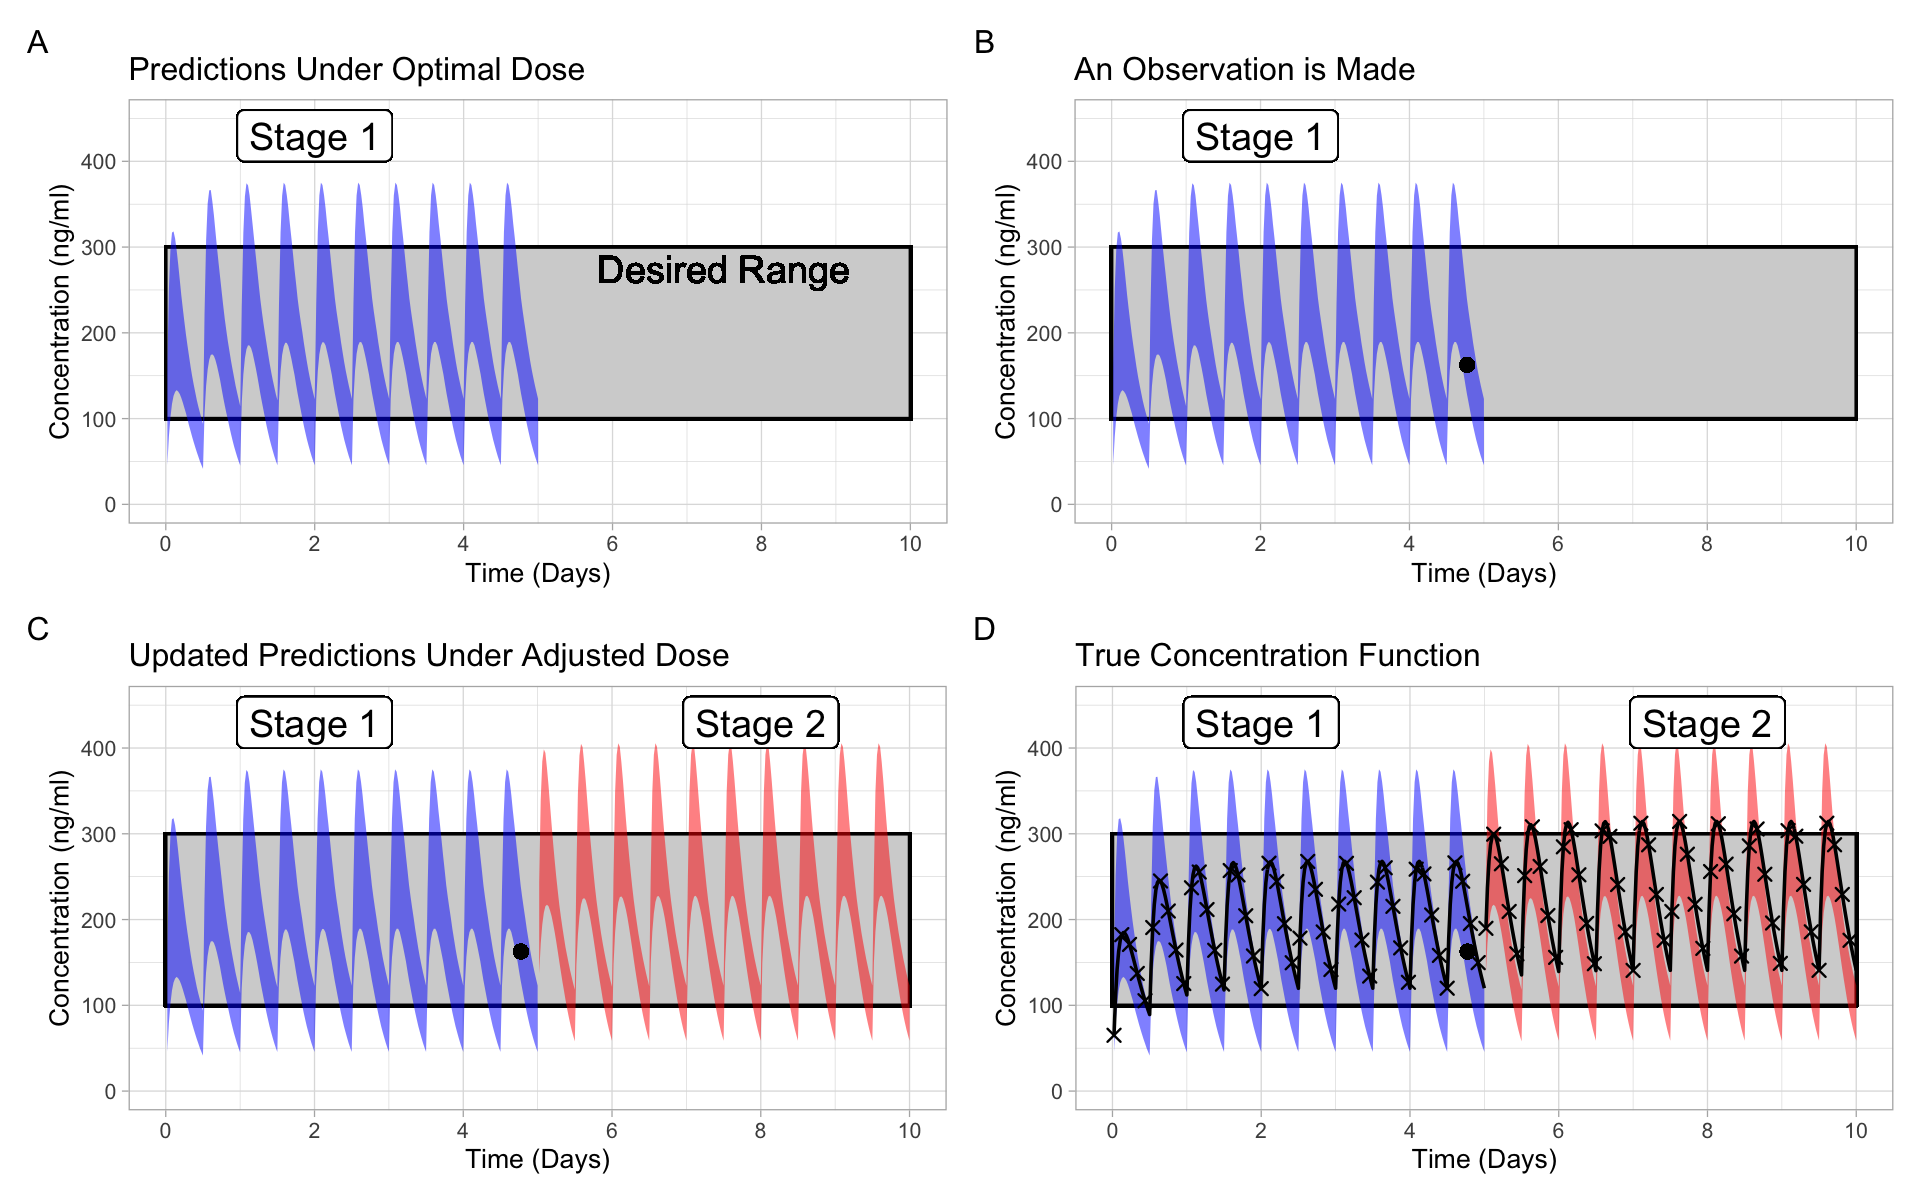
\includegraphics[width=1\linewidth]{figures/viz_of_process.png}
	\caption{
	Visual representation of the steps in our framework.	\textbf{A}  Using only clinical information, the model is used to select a dose to keep the patient in the desired range for as long as possible. The blue ribbon indicates 90\% credible interval for the latent concentration.  \textbf{B} Some time later, the patient's blood serum concentration is measured (black dot). \textbf{C}  The observation is incorporated into the model and a new dose is selected to keep the patient in range for as long as possible. The red ribbon indicates 90\% credible interval for the latent concentration after adjusting the dose. \textbf{D} The black line indicates the true latent concentration under each dose.  Note the observation (black dot) is not on the black line (true concentration) because there is measurement error, which the model accounts for.  Black exes indicate a discretization use to compute the reward function in each stage.
}
	\label{fig:processfiguresingle}
\end{figure}


	\section{Case Study}\label{ss:casestudy}

In this section, we present the results of applying our framework to investigate the potential benefits of static and dynamic personalization of apixaban dosing. Apixaban is a direct acting anticoagulant medication used to treat active blood clots occurring with deep venous thrombosis or pulmonary embolis, or to prevent stroke in patients with atrial fibrillation. Prescribing an apixaban dose that achieves blood concentrations within an optimal range is expected to provide optimal treatment benefits while minimizing harms (e.g., serious bleeding) for a drug considered to have a narrow therapeutic index. Indeed, patient-related factors that would predict high blood concentrations of apixaban such as age>80 years-old, weight <60 kg and kidney dysfunction are clinical variables that are normally considered in initial drug dose decisions. Additionally, female sex, comedications and genetic factors contribute to higher circulating apixaban concentrations \cite{gulilat2020drug}. These patient-related variables only explain 35\% of the pharmacokinetic variability in apixaban, which serves as rationale for dynamic dose optimization supported by post-initiation blood concentration monitoring. 
\subsection{Bayesian Modelling}

To create the necessary model for apixaban personalization, we extend a previously proposed one-compartment Bayesian pharmacokinetic model \cite{pananos2020comparisons} to include fixed effects of covariates on pharmacokinetic parameters in order to incorporate baseline clinical information (age, sex, weight, and creatinine.)  Full details of the model structure are provided in Appendix~\ref{ap:appendix}. We fit the model to previously-collected data on apixaban concentration \cite{tirona2018apixaban} and then use the fitted model to simulate patients with known "ground truth" pharmacokinetic parameters as described previously. We then use this population of simulated patients in our experiments to explore different modes of dose personalization and their relative benefits.

\begin{figure}
	\centering
	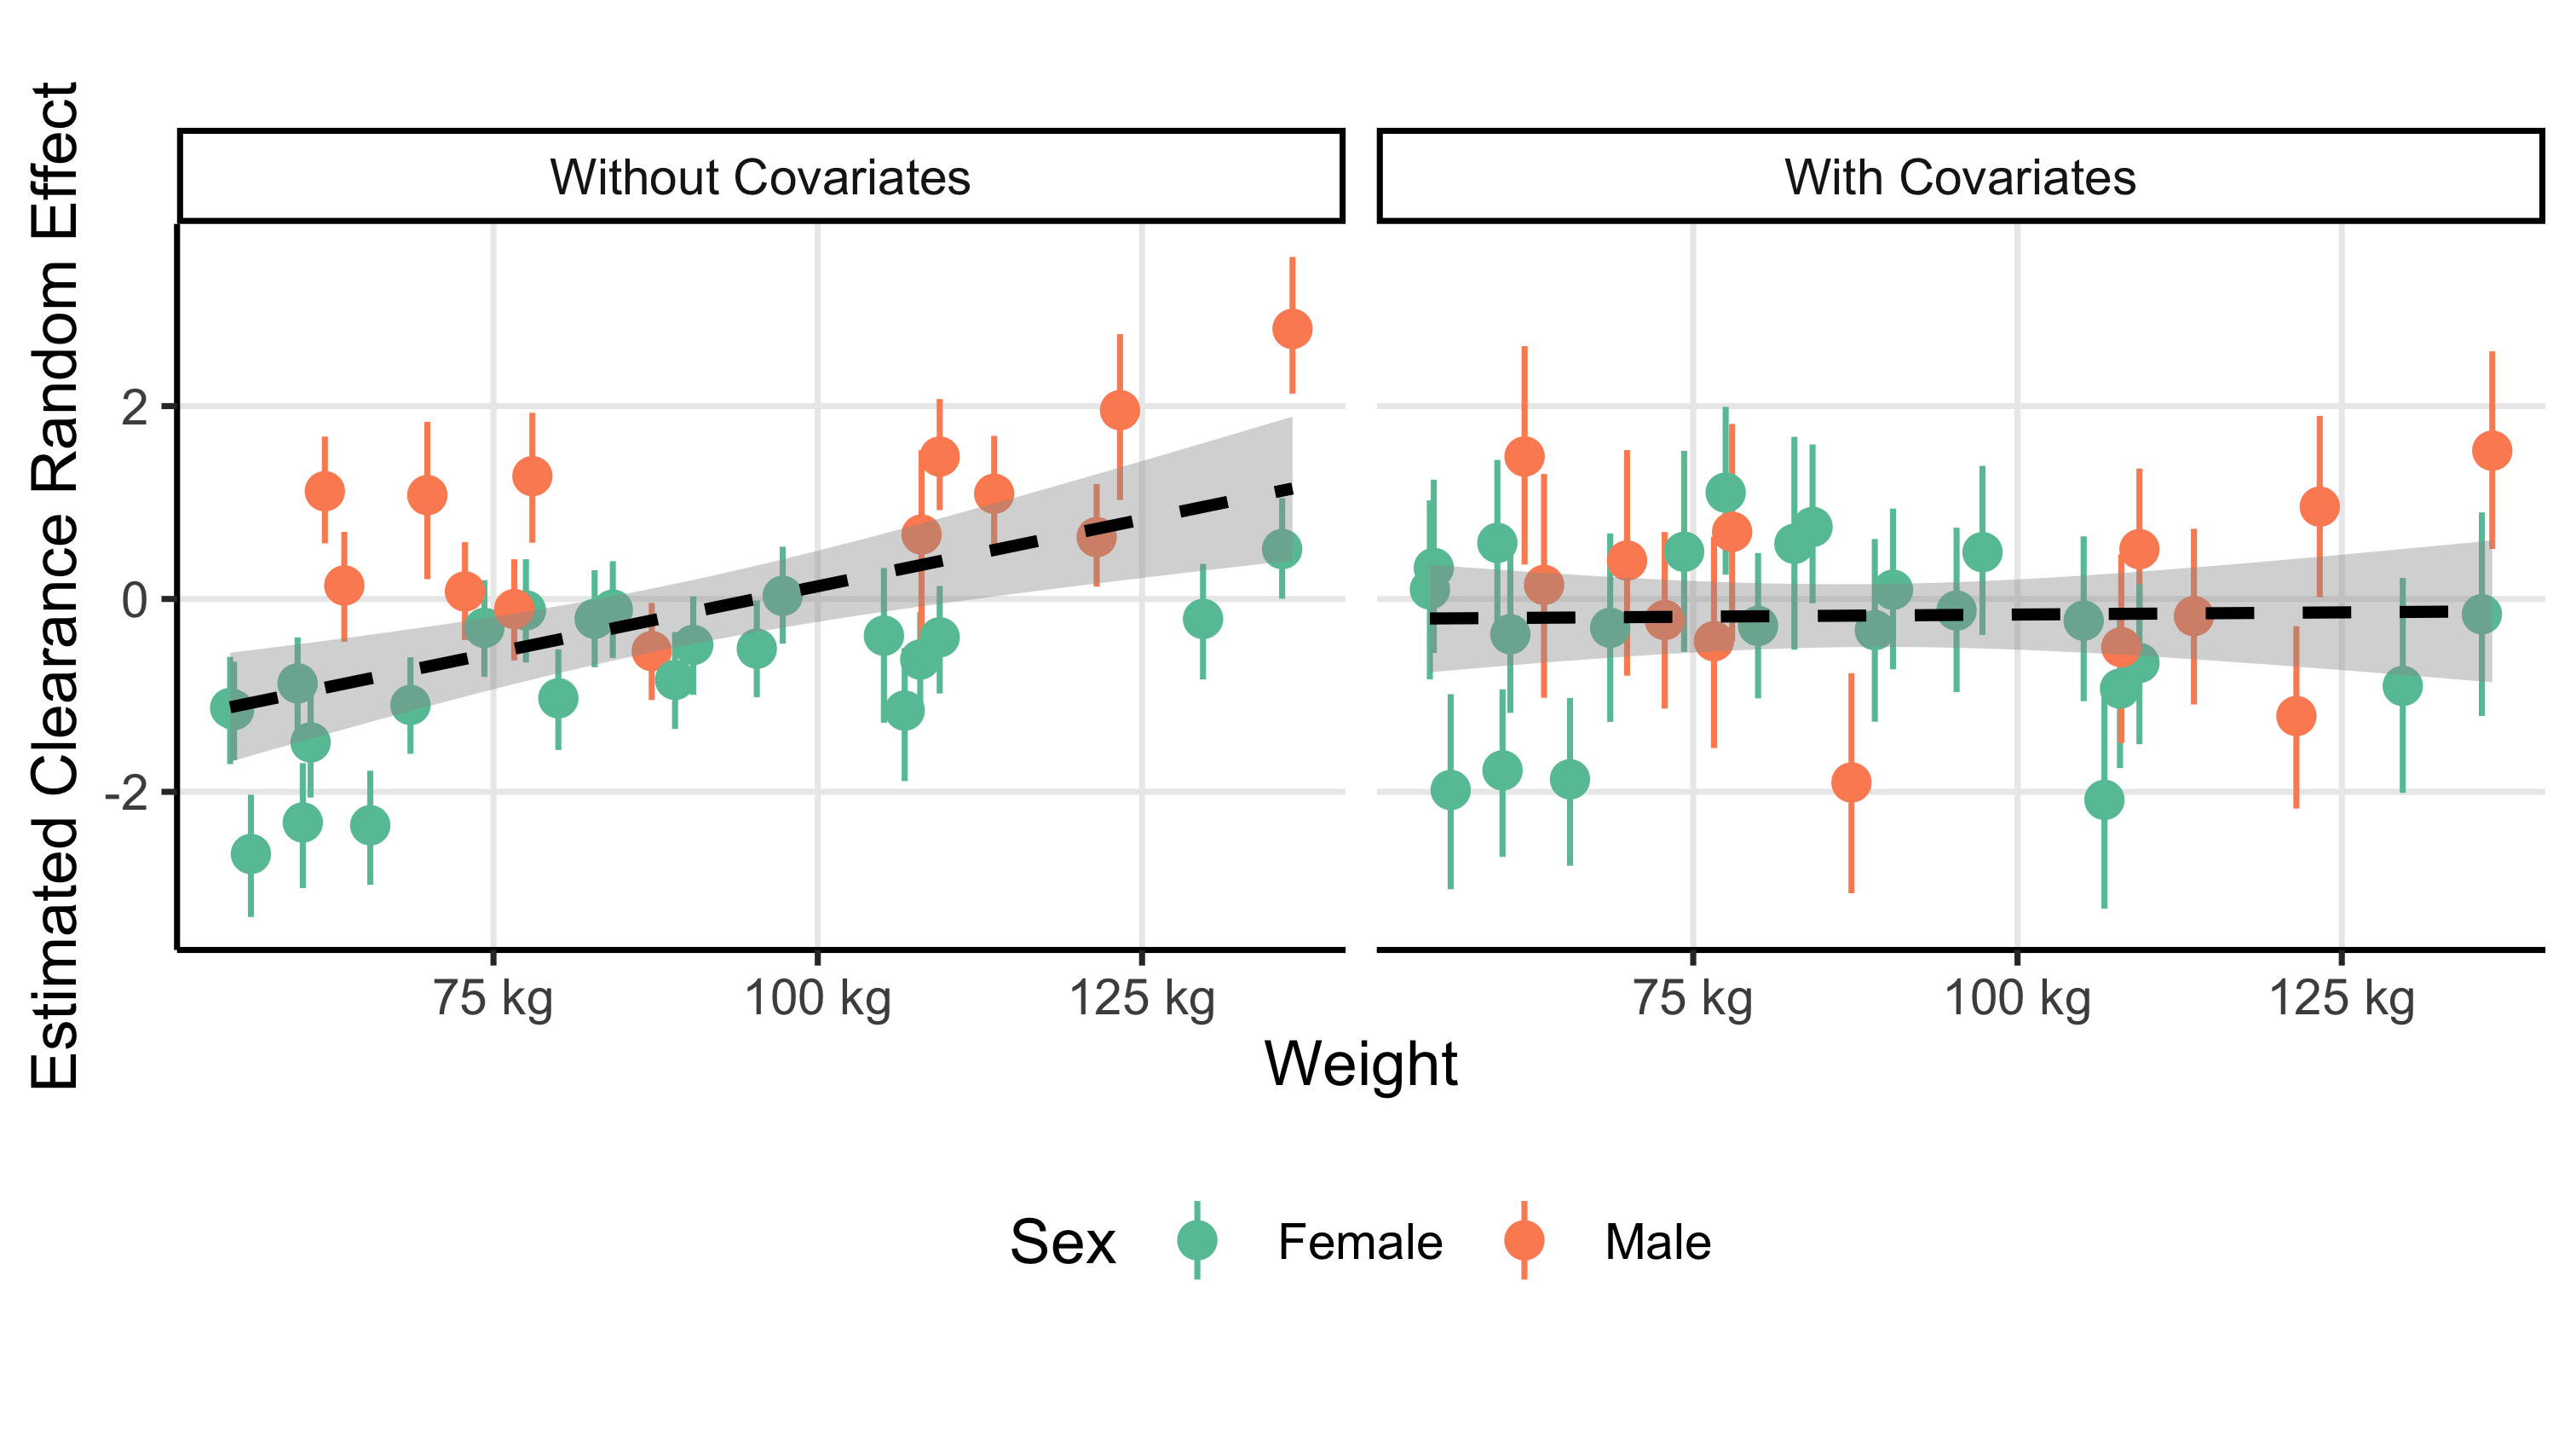
\includegraphics[width=\linewidth]{"figures/random_effects_change.png"}
	\caption{Random effects estimates for clearance $ CL_i $ and 95\% credible intervals (left).  Random effects estimates are colored by patient sex.  Prior to adjusting for covariates, a general trend in weight can be seen in the random effects.  Subjects who are heavier tend to have larger random effect, and males tend to have larger random effects than females of the same weight.  Patterns such as these indicate that weight and sex can be used to explain variation in the random effects.  After adjusting for sex and weight (right), the random effects have no discernable pattern.}
	\label{fig:randomeffectschange}
\end{figure}

We fit our model to real pharmacokinetic data using the open source probabalistic programming language, Stan \cite{gelman2015stan}.  Stan monitors several Markov chain diagnostics, none of which detected problematic Markov chain behavior, which indicates that Stan’s sampling algorithm was able to converge (0 divergences, all all Gelman-Rubin diagnostics<1.01, all effective sample size ratios  > 22\%).  

The inclusion of covariates in the model results in a better fit than excluding them. Shown in \cref{fig:randomeffectschange} are the estimated random effects for the clearance pharmacokinetic parameter of each subject as a function of weight.  Subject sex is indicated by color, the overall trend is shown in the black dashed line.  Failing to include subject sex and weight results in males having on average a larger random effect than females of the same weight, and heavier subjects having a larger random effect than lighter subjects.  When covariates are added into the model, the variation in the random effects attenuates, resulting in closer alignment to model assumptions. A better fit to the data means data generated from the model may be closer aligned with the true data generating process.

st order one compartment PK model.  The parameter $ \alpha $ is the ratio of how fast the drug exits the central compartment  how fast the drug enters the central compartment) which impacts the time to maximum concentration after each dose.  There is an estimated effect of sex on $ \alpha $ (males have smaller alpha than females, meaning the drug leaves their central compartment slower or enters the central compartment quicker), however the uncertainty is large (estimated effect -0.2 on the logit scale, 95\% credible interval -0.53 to 0.15). See \cref{tab:coefs} in the Appendix for a full summary of the regression coefficients.


%\begin{figure}
%	\centering
%	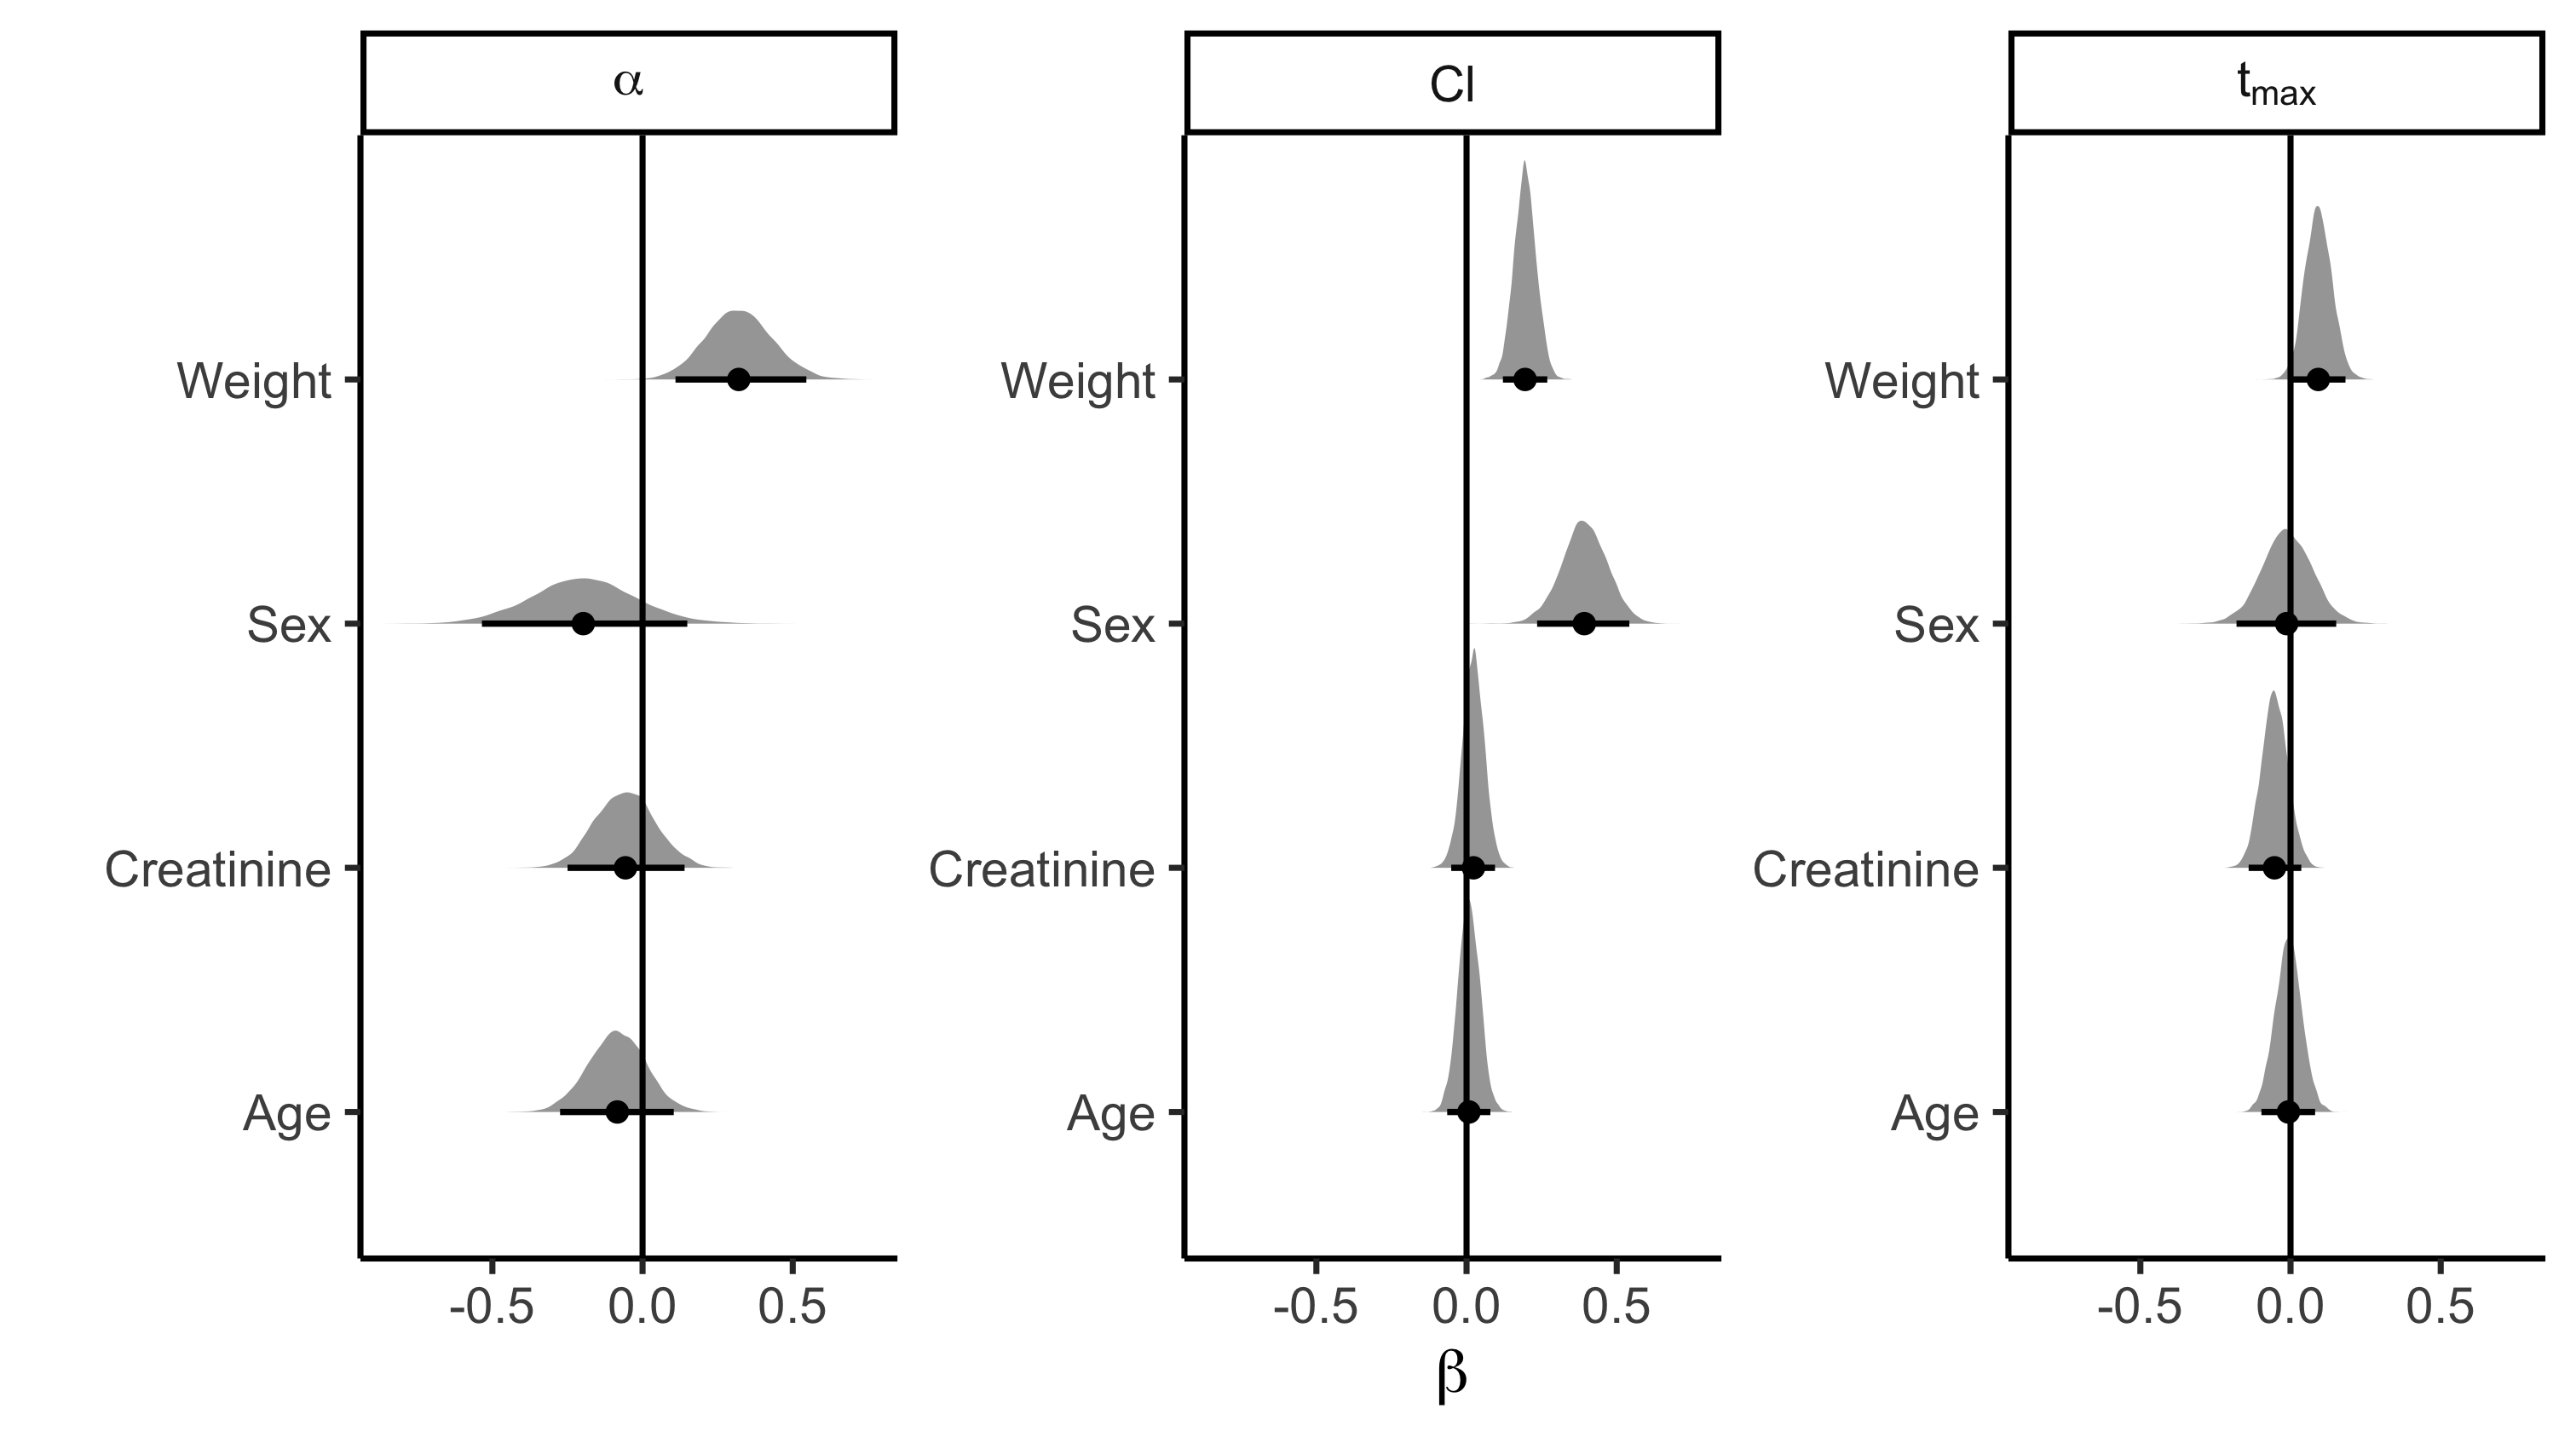
\includegraphics[width=1\linewidth]{figures/coef_vals}
%	\caption{Posterior distributions of regression coefficients. Expectations are shown as black dots, 95\% credible intervals are shown as horizontal black lines.  Solid black vertical line is $\beta=0$ for reference.  Note, regression coefficients for $Cl$ and $t_{max}$ act multiplicatively (a one unit increase in weight leads to a change in $Cl$ of $\exp(\beta)$), while regression coefficients for $\alpha$ are interpreted on the log odds scale.}
%	\label{fig:coefvals}
%\end{figure}


Model training error is comparable between the two models; the model without covariates achieves an average error of 8.31 ng/ml as measured by root mean squared error.  The model with covariates achieves a root mean squared error of 8.36  ng/ml.  Estimates of concentration uncertainty remain similar between the two models as well.  We conclude the inclusion of covariates in the model improves model inferences but does not substantially improve the fit of the model in this case.




\subsection{Modes of Personalization}



%\textcolor{red}{Make these descriptions "line up" with modes in Section 3? Break out into "static" and "dynamic"?}
%\begin{enumerate}[1)]
%\item Dose selection using a hierarchical Bayesian model which does not incorporate subject covariates.  This model was presented in Pananos \& Lizotte \cite{pananos2020comparisons}.  We refer to this mode as the “No Covariate Model”.
%\item 1) and conditioning the model on a single sample from the subject taken sometime in the final 12 hours before the half way point.  At the start of the fifth day, a new dose is selected and used for the remaining time.  We refer to this mode as “No Covariate + 1 Sample”.
%\item Dose selection from M2.  A single dose is selected at the start of the regimen and is used throughout the 10 simulated days. We refer to this mode as “Covariate Model”.
%\item 3) and conditioning the model on a single sample from the subject taken sometime in the final 12 hours before the half way point.  At the start of the fifth day, a new dose is selected and used for the remaining time. We refer to this mode as “Covariate model + 1 Sample”.
%\item A two stage DTR, however the initial dose is the result of the procedure in 3).  The best time to sample the patient is then determined via Q learning. We refer to this mode as “Optimal Sampling Time”.
%\item A two stage DTR estimated via Q learning.  We refer to this mode as “Q Learning”.
%\end{enumerate}

We consider the  6 modes of personalization as outlined in \cref{ss:framework}.  To evaluate these modes of personalization, we generate 1000 simulated subjects taking a dose of apixaban once every 12 hours with perfect adherence for a total of 10 days. The goal is to maximize the time spent with blood concentration level between between 100 ng/ml and 300 ng/ml. We choose this range as it is not so narrow that even optimal doses perform poorly, but not so wide that any dose can achieve high reward. For static modes of personalization, the selected initial dose is fixed over the 10 day period. For dynamic modes of personalization, some time in the second 12 hour period on the fourth day (between 108 and 120 hours after the initial dose), the simulated subject’s blood concentration is measured, and then at the start of the fifth day, the dose is adjusted based on all the pre-dose clinical measurements plus the observed concentration by incorporating information into the Bayesian model. 

\subsubsection{Defining the Dynamic Treatment Regimes}

To implement the two dynamic modes of personalization, we estimate DTRs with two stages (the first five days, and the latter five days).  For the dynamic personalization policies our experiments, we develop a DTR for selecting the best dose for keeping a patient’s blood plasma concentration within a desired range.  In terms of the DTR, the system is the patient for whom a dose is selected, the actions correspond to selection of dose sizes (and a time in the future to sample the patient, should the DTR require that), and the reward is the proportion of time spent within the desired concentration range. The trajectories we will use to estimate the optimal Q functions are of the form

\begin{equation}\label{key}
O_1, A_1, Y_1, O_2, A_2, Y_2
\end{equation}

\noindent The interpretation of a given trajectory is:
\begin{itemize}
	\item $ O_1 $ is any pre-dose clinical measurements of the subject.  In our experiments, we consider age in years, renal function (as measured by serum creatinine in mMol/L), weight in kilograms, and dichotmous biological sex (dummy coded so that male=1 and female=0).  We choose these variables as they are known to affect the pharmacokinetics of apixaban \cite{byon2019apixaban}.  
	\item $ A_1 $ is the initial dose to provide the subject.  If the DTR allows us to specify a time in the future at which to measure the subject’s blood serum concentration, then $A_1$ is the dual action of initial dose plus a time in the future at which to measure.
	\item $ Y_1 $ is the proportion of time spent within the concentration range in the first five days.
	\item $ O_2 $ is the pre clinical measurements of the subject plus the observed concentration made on the fourth day.
	\item $ A_2 $ is the dose adjustment
	\item $ Y_2 $ is the proportion of time spent within the concentration range in the final five days after the dose adjustment.
\end{itemize}

The actions $A_j$ effect the reward $Y_j$ by directly changing the concentrations at a given time.  For example, a larger dose will elicit larger concentrations which may put the patient in range for longer (more reward) or make take them out of range for some time (less reward).  Thus, our reward function can be thought of as a composition of the reward function and the concentration function.  In our experiments, we create a mesh of $2K$ times at which we can evaluate the latent concentration and compute the reward function.  Each stage in our DTR consists of $K=240$ times (equivalent to evaluating the latent concentration function every 30 minutes after ingestion).  Let $ c_i \>,  i=1...K \>, $ be the $ i^{th}$ latent concentration value at time $ t_i $.  The reward function in the first stage is

\begin{equation}
Y_1(H_1, A_1) = Y_1(c_1(A_1), \dots, c_K(A_1)) = \dfrac{1}{K}\sum_{i=1}^K \mathbb{I}(0.1 < c_i(A_1) < 0.3)
\end{equation}



\noindent Here, $ \mathbb{I} $ is an indicator function returning 1 if $c_i$ is between 100 ng/ml and 300 ng/ml and 0 else.
%To leverage off-the-shelf optimization tools, we approximate this reward function with a continuously differentiable function, namely
%\begin{equation}
%Y(c_1, c_2, \cdots,  c_k) = \dfrac{1}{k}\sum_{j=1}^K \exp\left( - \left[ \dfrac{c_j-0.15}{0.05} \right]^{2\beta} \right)
%\end{equation}
%
%\noindent Here, $ \beta $is a positive integer.  For sufficiently large beta, our approximation becomes arbitrarily close to our intended reward function.  In practice we set beta=5 to balance between good approximation of our intended reward and vanishing gradients impeding our optimization. 
%We suppress the dependence on the history in the definition of the reward as the reliance on the history is implicit.  The reward depends on the latent concentrations which depend on previous doses (actions) and potentially on the previous dose measurements (observations of the system).  We approximate this reward function with a continuously differentiable function to facilitate optimization.  See the appendix for details.  
\noindent The reward function in the second stage is

\begin{equation}
Y_2(H_2, A_2) = Y_1(c_{K+1}(A_2), \dots, c_{2K}(A_2)) = \dfrac{1}{K}\sum_{i=1}^K \mathbb{I}(0.1 < c_{K+i}(A_2) < 0.3)
\end{equation}



Our stage 2 optimal Q function is then

\begin{equation}
Q_{2}^{o p t}\left(H_{2}, A_{2}\right)=E\left[Y_2\left(c_{K+1}(A_2), \cdots, c_{2K}(A_2)\right) \Bigg\vert H_{2}, A_{2}\right] \>,
\end{equation}

\noindent and our stage 1 optimal Q function is

\begin{equation}
Q_{1}^{o p t}\left(H_{1}, A_{1}\right)= E \left[Y_1\left(c_{1}(A_1),  \cdots, c_{K}(A_1)\right)+\max _{a_{2} \in \mathscr{A}} Q_{2}^{o p t}\left(H_{2}, a_{2}\right) \Bigg\vert H_{1}, A_{1}\right]
\end{equation}

We seek to maximize the stage 1 optimal Q function to learn the optimal policy for dosing subjects under the constraint we can measure them at most once and are limited to the aforementioned pre-dose clinical variables.  The interpretation of stage 1 optimal Q function is as follows:\textit{ Given the pre-dose clinical variables of the subject and a proposed initial dose and measurement time, the stage 1 optimal Q function gives the proportion of time the subject’s blood serum concentration is between 100 ng/ml and 300 ng/ml assuming that we provide the subject with the best dose possible at the start of the $ 5^{th} $ day.}  The actions $ A_1 $ and $ A_2 $ which maximize these functions constitute the optimal policy.


%
%The concentration values $ c_j $ in the optimal Q functions are latent, meaning we have no direct access to them in practice. Furthermore, obtaining measurements with high enough frequency so that the reward is faithfully estimated would be too burdensome on the patient. 


\subsection{Evaluation}

We present the results of our simulation in \cref{fig:modelsofpersonalizationdifferences} below in terms of difference between theoretically largest reward and reward achieved by the mode of personalization.  The results are ordered from least amount of information and burden (top) to most amount of information and burden (bottom) and colored by their personalization strategy (static or dynamic).

Modes of personalization which use less information have a larger difference (i.e. yield smaller reward on average than what is theoretically possible).  The One Size Fits All approach (which uses no information about the subject) performs worst with a median difference of 0.145.  The distribution of differences for this mode is right skewed with some differences exceeding 0.95, meaning the subject could have been in range for nearly the entire time but the mode selected a dose which failed to put the subject in range. 

The use of clinical variables in the model nearly cuts the difference in half, achieving a median difference of 0.086 with smaller right skew.  There is a diminishing in the difference in rewards as additional burden is undertaken. Modes which use observed concentration information (Clinical Variables + One Sample, Optimal Sampling Time, and Optimal Sequential Dosing) lead to marginally lower median differences  (0.075, 0.076, 0.079 respectively) as compared to the use of clinical variables alone.


\begin{figure}
	\centering
	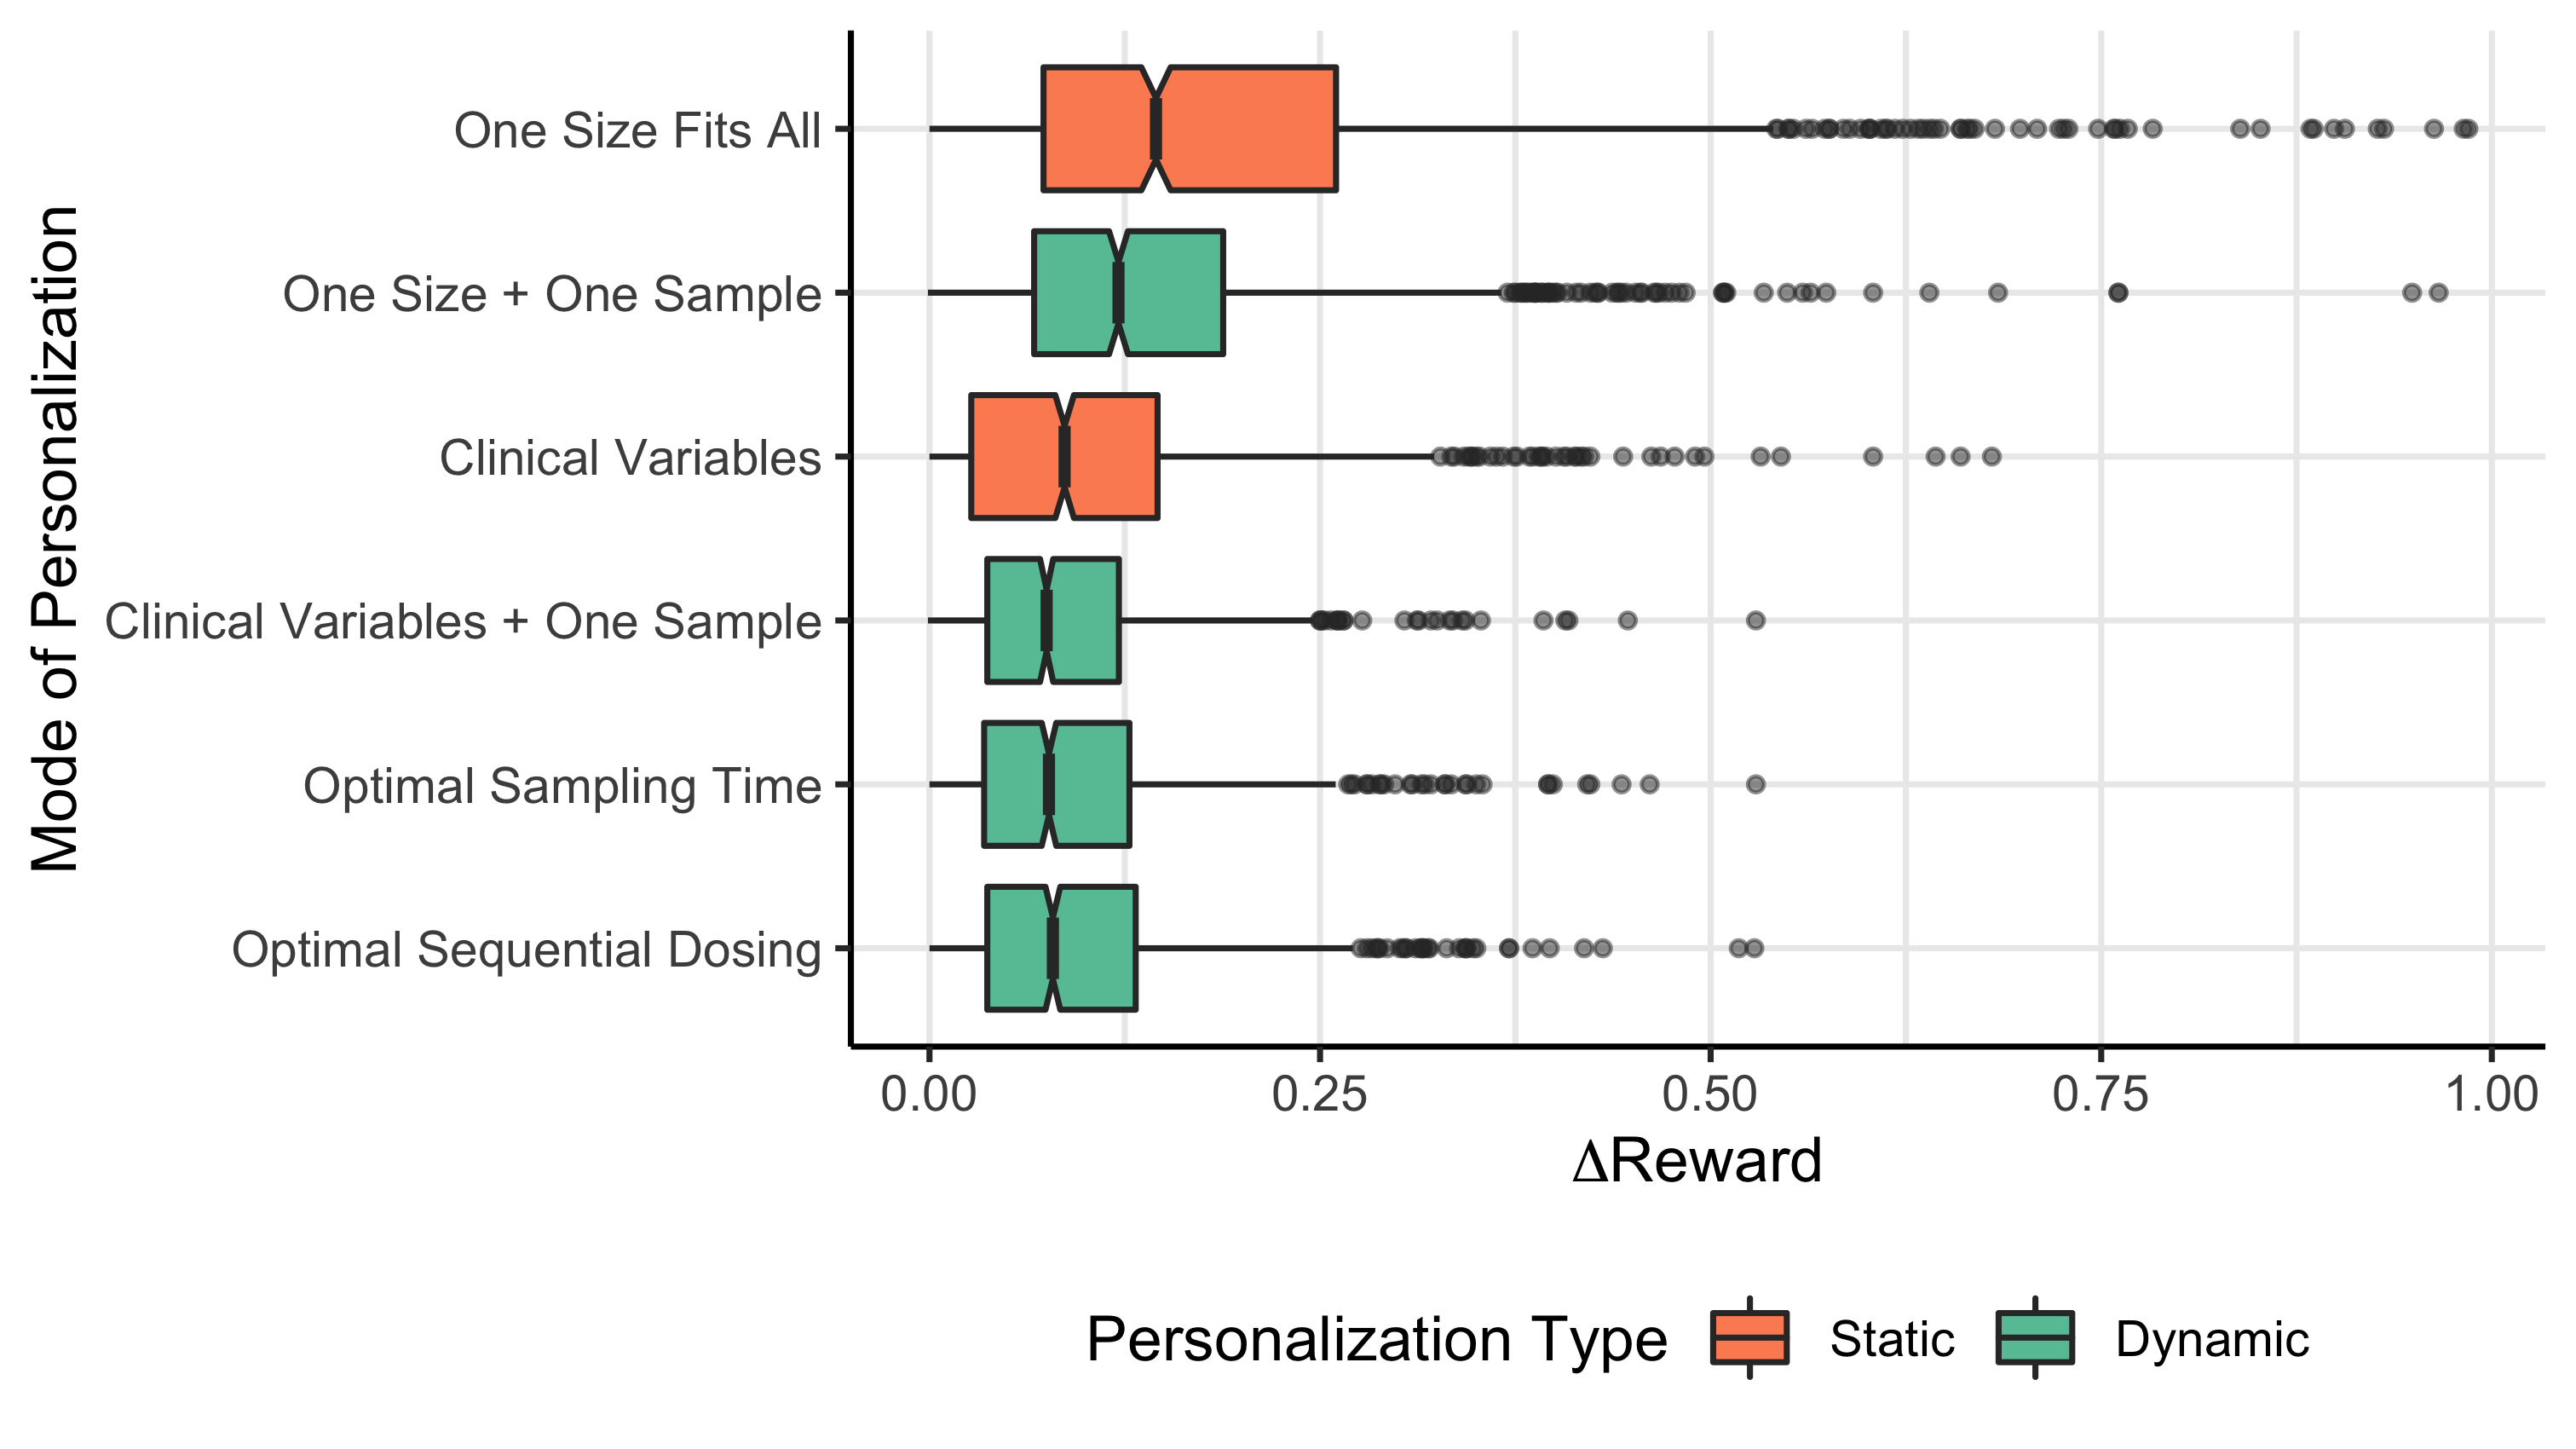
\includegraphics[width=1\linewidth]{figures/models_of_personalization_differences}
	\caption{Boxplots of the difference between theoretically largest reward and achieved reward for each of the 1000 simulated subjects. Subjects who achieve a reward close to their maximium reward have a difference on 0, subjects who achieve a reward less than their maximum have larger differences, with the largest difference being 1.}
	\label{fig:modelsofpersonalizationdifferences}
\end{figure}

	\section{Discussion}\label{ss:discussion}

%Including age, sex, weight, and creatinine in our Bayesian model improved the inferences from that model.  Though the predicted concentrations and estimates of uncertainty changed negligibly, the covariates explained residual confounding in the random effects. This results in a model which better explains the observed variation in the data and hence should generate more plausible data for simulation.

In the following, we discuss the results of our case study, followed by a discussion of the broader potential implications of personalized medicine policy.

%Working subsection titles - not sure if they stay
\subsection{Comparing Modes of Personalization}

As expected, modes of personalization which use more information result in larger reward. However, if we consider the expected reward of the different modes, there is diminishing return on investment observed when using additional information from observations of blood concentrations (and consequently, taking on additional implementation burden to effectively use that information). 

%\textcolor{red}{I wonder if we can make a clearer, more quantitative argument in terms of why. One way is to make it conditional -- if we care about xx the most, then we would do yy. On the other hand, if we care about yy, maybe we would do... This is easier to sell than "I would recommend this." You can even phrase it as like, unless you care super a lot about that last 1\% of reward, realistically you should just do xx. So, this is just about framing.}Were doses to be personalized for the simulated population, we would recommend the covariate model be used, as it is easier to implement, puts smaller burden on the clinic, and results in approximately mean/median rewards as compared to other methods.  Taking an additional sample doesn’t seem to improve the expected mean/median reward appreciably to be worth the burden of having the patient take time to come in, drawing their blood, measuring their concentration in the lab, and reporting results to the decision maker, in which a decision to not adjust the dose might be made anyway. Similar arguments can be made for Q learning, which has even higher implementation burden.


If investigators were interested in deploying personalization of apixaban in the population of patients which generated the data used to fit our models, then the Clinical Variables mode balances relatively low implementation burden with high reward. However, deploying the Clinical Variables mode of personalization comes with the consequence of larger right skew of difference betwen largest and achieved reward.  This means that while the majority of patients will achieve a reward near what is hypothetically largest, there is increased risk that a patient will achieve less than half of their theoretically largest reward, comparitvely speaking.  If avoiding this possibility is of interest to investigators, then taking on additional implementation burden of collecting additional samples from patients to reign in the right tail of the distribution of differences via the Clinical Variables + One Sample mode may be the way forward.  The performance of the Clinical Variable mode in these experiments is due to the fact that the variables included in the model are known to affect the pharmacokinetics of apixiban.  In cases where clinical variables are not as predictive, then the we would expect the Clinical Variables model to have higher median/mean differences.  Dynamic personalization via collecting additional samples would then have a bigger advantage relative to static personalization.

In our experiments, the dynamic modes of personalization (Clinical Variables + One Sample, Optimal Sampling Time, and Optimal Sequential Dosing) all performed similarly and any differences would not be considered statistically or practically significant.  However, that is not to say that there may not be different contexts for other drugs for which differences may be observed.  After ingestion and absorption, the concentration of apixiban in the blood looks approximately like $e^{-k_e t}$ (up to a constant).  Thus the change in concentration from hour to hour can be relatively quick or prohibitively slow, depending on the size of $k_e$.  In cases where $k_e$ is small, eliminating a dose which is too big will take time and can keep patients out of a desired range for extended periods even after adjustment to a more appropriate dose.  Hence, in cases like these the Optimal Sequential Dosing mode might be more preferable, even at the cost of the largest implementation burden, as it can more effectively balance the exploration and exploitation via optimization of Q functions.

It is clear that there are tradeoffs between achieving a reward close to what is theoretically largest and taking on additional clinic and implementation burden, and that tradeoff should be examined on a case-by-case basis.  Context is crucial, and how we adapt to that context is perhaps a question in need of closer examination.  Traditional methods of personalization include conditioning only on a subject’s covariates (not unlike the Clinical Variables mode we present here).  But of course patients are not their age, sex, weight, and creatinine.  Additionally, safety information and best available practices might change in the future as more research on drugs is performed. Were new safety information to be published, one might imagine the reward function might be affected, which may result in a new mode of personalization being more/less preferable or more/less feasible.  Any number of factors in flux can change the context in which personalization occurs, and that change in context may prompt for a re-evaluation in how personalization is done.

We do not offer recommendations on how personalization for apixaban should be done because this depends on the context of the health system and population where such personalization would be deployed. Rather, we offer  a framework for developing strategies of personalization and evaluating their performance against their implementation and patient and provider burden.  Context can be changed where needed, either through the reward function, or by adjusting when the clinic is able to take measurements, or by including additional information such as genotype in the Bayesian model.  Using this framework, clinics have flexibility to personalize the personalization.


%Working subsection titles - not sure if they stay
\subsection{Relating Results to Policy Decisions}

Personalized medicine still faces several barriers to widespread adoption, including economic burden, patient burden, and expertise burden required for new methods of personalization.
Personalized medicine can increase safety and reduce costs to the healthcare system by identifying patients who are at greater risk for adverse events or dose adjustments.  For example, if personalization enables a patient to avoid an adverse event, then this avoids associated costs to the healthcare system, example from a hospital stay \cite{looff2016economic}.  More ambitiously, personalized medicine has the potential to save the healthcare system costs by more effectively using resources \cite{shabaruddin2015economic}. 

The cost of patient testing and monitoring, personnel, and training  required to operate a personalized medicine clinic are high burden, and it is not yet clear if personalized medicine is sufficiently cost effective to offset operating costs in all circumstances \cite{kasztura2019cost}.  In their 2019 scoping review of personalized medicine cost effectiveness, Kasztura et. al \cite{kasztura2019cost} found that willingness-to-pay thresholds vary wildly from country to country (citing that cost per quality adjusted life year for some modes of personalized medicine range from \$20,000 USD per quality adjusted life year in for studies in Europe and the United Kingdom to \$200,000 USD per quality adjusted life year for studies in the United States).  This high variability in cost effectiveness means the burden required for start up may result in a positive return on investment in some areas but not others. This variability should prompt would be adopters to more closely examine if taking on the initial burden is worth the result.

% beef up here
% Examples.  Identifty clear examples from the literature around diagnostics?
The dominant perspective on personalized medicine focuses on the use of clinical and physiological information (including biomarkers, genotyping, and diagnostic tests) as a means of optimizing treatments, but largely ignore needs, constraints, and utilities of the patient \cite{rogowski2015concepts, di2017personalized}. Patients can be burdened by frequent followup for clinical measurement (as in the case with warfarin), be burdened by costly expenses related to obtaining care, or may be more risk adverse/tolerant than the ``typical'' patient. As an example, transportation has been found to be a large financial burden for patients receiving cancer treatment \cite{houts1984nonmedical}, and continues to burden patients, with a 2020 study finding that the cost of parking alone can climb as high as \$1600 over the course of treatment in the United States \cite{lee2020assessment}.  Additional visits to a clinic have the potential to further burden patients by requiring them to miss a day of work, and find means of childcare during their absence (if necessary). Incorporating patient preferences and reducing the burden of personalization on the patient can result in sustained adherence \cite{elliott2008understanding}, thereby increasing effectiveness and further preventing adverse events.

% FInd some machine learning cautinary tales

An additional expertise burden is added as machine learning (used interchangeably with the term “artificial intelligence”) is adopted into personalized medicine initiatives.  Cutting edge machine learning models for prediction or decision making can be prohibitively burdensome to implement effectively. Failure to carefully implement a prediction model may result in pernicious bias inadvertently affecting subpopulations, as was found to be the case in algorithms for credit scoring \cite{barocas2016big}, crime prediction \cite{lum2016predict}, and hiring \cite{ajunwa2020paradox}.  A 2019 study found an instance of this bias in a widely used risk scoring algorithm in healthcare \cite{obermeyer2019dissecting}, demonstrating that despite the best intentions of those involved, the use of a model can lead to worse rather than better care if investigators are not careful in considering what sorts of bias may be present in the data used to train these models.  Implementation of new approaches and methods requires the close collaboration of experts in data science  with physicians, domain experts, and other stakeholders.  Close collaboration should allow for domain experts to identify what kinds of biases the data might have, and for data science experts to implement methods to help ameliorate that bias (or to admit the data are not fit for purpose).  The result of iterating on this collaborative process (wherein domain experts help inform the appraoches methodologists take, and the methodologists provide model checks which help domain experts decide if decisions from the model are reasonable or suspicious) is a model which more closely aligns with domain expertise, a model which is sufficiently flexible to capture the true data generating mechanism, an effective use of data, a more transparent modelling process, and calibrated expectations surrounding algorithms and their abilities \cite{frohlich2018hype}.  Presently, this form of collaboration between methodologists and domain experts is not the norm, with development of machine learning solutions in healthcare being developed in silos \cite{wiens2019no}.  These burdens may be surmountable for some, but the question then turns to if the result is worth the expense.   Answering that question is difficult without an idea how the additional burden of collecting data, or implementing new algorithms, will benefit the clinic or the patient subject to inherent constraints. 



Implementation decisions made at the organizational level need to attend to a broad array of evidence and contextual factors. Know4Go \cite{martin2016hospital} is one such framework for explicitly considering factors from expanded domains of influence surrounding adoption of new technologies/interventions in a healthcare setting (like a clinic or hospital). These expanded domains of influence include: social, legal, ethical, environmental/institutional, political, entrepreneurial/innovative, research opportunity, and reversibility factors in conjunction with objective evidence of benefits versus risks, systematic review, and costs.  Broadly, once evidence has been synthesized through systematic review and/or meta-analysis, the evidence is contextualized to local healthcare system perspective.  Evidence is converted onto a benefit scale, derived from the number of patients likely to benefit from adoption of the technology/intervention.  Budget impact of the adoption is estimated using costing data from the hospital/clinic, and new technologies can be triaged according to their impact and cost.  Our framework could produce benefit evidence that is used in the Know4Go framework to inform organization-level decisions surrounding implementation of personalization.


\subsection{Limitations}

We’ve examined six modes for making decisions.  The next mode improves on a deficiency of the previous mode in a natural manner, and so our experiment constitutes a kind of ablation study.  We believe the decision making aspect of our study extracts information in a responsible way and uses the best decision making methodology available.  That being said, the experiment is not without limitations.

The Bayesian model of the pharmacokinetics is integral to the methodology we present.  Any shortcomings in the model affect the quality of the decision and decision process.  Bayesian models are not as ubiquitous as other models in pharmacology, and so particular expertise is required for model development and evaluation.  That expertise increases the implementation burden of any decision process involving Bayesian models.  However, we demonstrate how one such model can be constructed in a past study \cite{pananos2020comparisons} and include open sourced code and data for practitioners to replicate our model fitting.

Additionally, the data required to construct a high quality Bayesian model of pharmacokinetics require multiple observations of a single patient over an extended time, preferably over multiple well timed doses with near perfect adherence.  Obtaining such data requires well organized efforts and is high burden for both investigators and participating subjects.  This makes acquiring a robust Bayesian model for use in dose personalization difficult.



\subsection{Future Work}

Because the data required to build reliable Bayesian pharmacokinetic models are difficult to collect in practice, research into developing these models from observational data may prove fruitful in extending this work. If clinics record data on measured blood concentrations, they may have dozens or hundreds of subjects with only one or two measurements per subject.  Moreover, the subjects in question may be on multiple drugs or have comorbidities which may affect the pharmacokinetics of the drug under study.  Additional research into constructing Bayesian models which can adjust for polypharmacy and comorbidities while learning an individual’s pharmacokinetics from a large but sparse sample would drive this work towards being easier to implement in practice.



	\newpage
	\bibliography{./bibs/introduction,./bibs/dtr, ./bibs/bayes}
	\newpage
	\appendix
	\section{Appendix}\label{ap:appendix}

\subsection{Model Details}

The Bayesian model used to predict personalized concentration in response to dose, which we refer to as $ \mathcal{M}_1 $, is 

\begin{align}\label{model_M1}
	y_{i,j} &\sim \Lognormal  \left(  C_i(t_j)  , \sigma^2_y \right)  \\
	\sigma^2 &\sim \Lognormal \left( 0.1, 0.2 \right)\\	
	C_i(t_j) &= \begin{dcases}
	\frac{D_{i} \cdot F}{C l_{i}} \cdot \frac{k_{e, i} \cdot k_{a, i}}{k_{e, i}-k_{a, i}}\left(e^{-k_{a, i}\left(t_{j}-\delta_{i}\right)}-e^{-k_{e, i}\left(t_{j}-\delta_{i}\right)}\right) & t_j>\delta_i \\
	0 & \mbox{else}
	\end{dcases}\\
	k_{e,i} &= \alpha_i \cdot k_{a,i}\\
	k_{a,i} &= \dfrac{\log(\alpha_i)}{t_{max, i}\cdot(\alpha_i-1)}\\
	\delta_i &\sim \operatorname{Beta}(\phi, \kappa) \\
	\operatorname{logit}(\alpha_i) \vert \beta_\alpha, \sigma^2_\alpha &\sim \Normal(\mu_\alpha + \mathbf{x}_i^T \beta_\alpha, \sigma^2_\alpha)\\
	\log(t_{max, i}) \vert \beta_{t_{max}}, \sigma_{t_{max}} &\sim \Normal(\mu_{t_{max}} + \mathbf{x}^T_i \beta_{t_{max}}, \sigma^2_{t_{max}}) \\
	\log(Cl_i) \vert \beta_{Cl}, \sigma_{Cl} &\sim \Normal(\mu_{Cl} + \mathbf{x}^T_i \beta_{Cl}, \sigma^2_{Cl}) \\ \nonumber \\
	p(\phi) &\sim \operatorname{Beta}(20, 20)\\
	p(\kappa) &\sim \operatorname{Beta}(20, 20)\\
	p(\mu_{Cl}) &\sim \Normal(\log(3.3), 0.15^2)\\
	p(\mu_{t_{max}}) &\sim \Normal(\log(3.3), 0.1^2)\\
	p(\mu_{\alpha}) &\sim \Normal(-0.25, 0.5^2)\\
	p(\sigma_y) &\sim \Lognormal(\log(0.1), 0.2^2)\\
	p(\sigma_{CL}) &\sim \Gmma(15, 100)\\
	p(\sigma_{t_{max}}) &\sim \Gmma(5, 100)\\
	p(\sigma_{\alpha}) &\sim \Gmma(10, 100)\\
	p(\beta_{Cl, k}) &\sim \Normal(0, 0.25^2) \quad k = 1 ...	 4\\
	p(\beta_{t_{max}, k}) &\sim \Normal(0, 0.25^2) \quad k = 1 ... 4\\	
	p(\beta_{\alpha, k}) &\sim \Normal(0, 0.25^2) \quad k = 1 ... 4
\end{align}

Here, normal distributions are parameterized by their mean and variance, lognormal distributions are parameterized by the mean and variance of the random variable on the log scale, and gamma distributions are parameterized by their shape and rate.  The $\mu$ in the model above represent population means on either the log or logit scale, the $\beta$ are regression coefficients for the indicated pharmacokinetic parameter, the sigmas are the population level standard deviations on the log or logit scale, $\delta$ is aparameter which relaxes the assumption that the dose is absorbed into the blood immeditately upon ingestion, $F$ is the bioavailability of apixiban (which we fix to 0.5 \cite{byon2019apixaban}) and $D$ is the size of the dose in milligrams.  All continuous variables were standardized using the sample mean and standard deviation prior to being passed to the model. 



\begin{table}\label{tab:coefs}
	\centering
	\begin{tabular}[t]{rccc}
		\toprule
		& $\beta_\alpha$ & $\beta_{Cl}$ & $\beta_{t_{max}}$\\
		\midrule
		\cellcolor{gray!6}{Age} & \cellcolor{gray!6}{-0.08 (-0.27,0.1)} & \cellcolor{gray!6}{0.01 (-0.06,0.08)} & \cellcolor{gray!6}{-0.01 (-0.1,0.08)}\\
		Creatinine & -0.06 (-0.25,0.14) & 0.02 (-0.05,0.09) & -0.05 (-0.14,0.04)\\
		\cellcolor{gray!6}{Sex} & \cellcolor{gray!6}{-0.2 (-0.53,0.15)} & \cellcolor{gray!6}{0.39 (0.23,0.54)} & \cellcolor{gray!6}{-0.01 (-0.18,0.15)}\\
		Weight & 0.32 (0.11,0.55) & 0.2 (0.12,0.27) & 0.09 (0.01,0.18)\\
		\bottomrule
	\end{tabular}
	\caption{Posterior means for coefficients for each covariate in our pharmacokinetic model.  In parantheses are 95\% credible interval estimates.}
\end{table}


Once fit, $ \mathcal{M}_1$ can be used to predict the pharmacokinetics of new patients, using the patient’s covariates as predictors.  To do so, the marginal posterior distributions for $ \mu_{Cl} $, $ \mu_{t_{max}} $, $ \mu_{\alpha}$, $ \beta_{Cl} $, $ \beta_{t_{max}} $, $ \beta_{\alpha} $, $ \sigma_{Cl} $, $ \sigma_{t_{max}} $, $ \sigma_{\alpha} $, and $ \sigma_y $ must be summarized.  We use maximum likelihood on the posterior samples to summarize the marginal posterior distributions. We model the population means  and regression coefficients as normal, and the standard deviations  as gamma.  The maximum likelihood estimates are used to construct priors for a new model, which we call $ \mathcal{M}_2 $. We construct $ \mathcal{M}_2 $ so as to be able to predict plasma concentration after multiple doses (of potentially different sizes) administered over time, and remove the time delay ($ \delta $) to simplify our simulations.  Model priors for $ \mathcal{M}_2 $ are then 

\begin{align}
	p(\mu_{Cl}) & \sim \Normal(0.5, 0.04) \\
	p(\mu_{t_{max}}) & \sim \Normal(0.93, 0.05) \\
	p(\mu_\alpha) &\sim \Normal(-1.35, 0.13)\\
									\nonumber \\
	p(\sigma_{Cl}) &\sim \Gmma(69.15, 338.31)\\
	p(\sigma_{t_{max}}) &\sim \Gmma(74.96, 349.56)\\
	p(\sigma_{\alpha}) &\sim \Gmma(10.1, 102.07)\\
									\nonumber\\
	p(\beta_{Cl, 1}) &\sim \Normal(0.39, 0.08^2)\\
	p(\beta_{Cl, 2}) &\sim \Normal(0.19,0.04^2)\\
	p(\beta_{Cl, 3}) &\sim \Normal(0.02,0.04^2)\\
	p(\beta_{Cl, 4}) &\sim \Normal(0.01,0.04^2)\\
									\nonumber\\
	p(\beta_{t_{max}, 1}) &\sim \Normal(-0.01, 0.08^2)\\
	p(\beta_{t_{max}, 2}) &\sim \Normal(0.09,0.05^2)\\
	p(\beta_{t_{max}, 3}) &\sim \Normal(-0.05,0.04^2)\\
	p(\beta_{t_{max}, 4}) &\sim \Normal(-0.01,0.04^2)\\
										\nonumber\\
	p(\beta_{\alpha, 1}) &\sim \Normal(-0.19, 0.17^2)\\
	p(\beta_{\alpha, 2}) &\sim \Normal(0.33,0.11^2)\\
	p(\beta_{\alpha, 3}) &\sim \Normal(-0.06,0.1^2)\\
	p(\beta_{\alpha, 4}) &\sim \Normal(-0.09,0.1^2)\\
\end{align}

For our experiments, we generate the pharmacokinetic parameters of 1000 simulated patients from the prior predictive model of $ \mathcal{M}_2 $. Bayesian models are generative models, meaning they can generate pseudodata by drawing random variables according to the model specification going from top (model priors) to bottom (model likelihood).  To do so, we begin by resampling 1000 tuples of age, sex, weight, and creatinine from the dataset used to fit $ \mathcal{M_1} $. We sample one draw of r $ \mu_{Cl} $, $ \mu_{t_{max}} $, $ \mu_{\alpha}$, $ \beta_{Cl} $, $ \beta_{t_{max}} $, and $ \beta_{\alpha} $  from their respective prior distributions in  $ \mathcal{M}_2 $. The values of these parameters remained fixed for all 1000 patients. Conditioned on the values of these mus and betas, we compute the expectation of the population distribution for each pharmacokinetic parameter by computing $ \mu_{Cl} + \mathbf{x}^T \beta_{Cl} $, $ \mu_{t_{\max}} + \mathbf{x}^T \beta_{t_{max}} $,  $ \mu_{\alpha} + \mathbf{x}^T \beta_{\alpha} $, where $\mathbf{x}^T$ is the resampled tuple.  From the prior distribution of M2, we sample one draw of$ \sigma_{Cl} $, $ \sigma_{t_{max}} $, $ \sigma_{\alpha} $, and $ \sigma_y $.  These remained fixed for all 1000 patients. Using the previously computed expectations and $\sigma$, we sample 1000 tuples of pharmacokinetic parameters, one for each of the simulated patients.  The clearance rate and time to max concentration were sampled assuming a lognormal distribution.  Alpha was sampled using a logitnormal distribution. The pharmacokinetics can then be determined conditional on the pharmacokinetic parameters. Each of simulated patients' pharmacokinetic parameters remained fixed through the experiments.  We simulate the latent concentration using $ C(t) $ as written in $\mathcal{M}_2$, and can simulate observed concentrations by drawing a sample from a lognormal distribution with mean $\ln(C(t))$ and standard deviation $ \sigma_y$

We use Stan, an open source probabilistic programming language, for fitting our Bayesian models via Hamiltonian Monte Carlo (a Markov Chain Monte Carlo technique) and computing markov chain diagnostics. Twelve chains are initialized and run for 2000 iterations each (1000 for warmup allowing the Markov chain the opportunity to find the correct target distribution and 1000 to use as samples from the posterior).


\subsection{Diagnostics For Bayesian Models Fit Via MCMC}

Once the form of the model is specified, creating simulated patients or estimating the PK parameters of a real patient requires computation of or sampling from the posterior distribution of the relevant variables given the relevant data. However, exact computation of the posterior distribution is intractable for all but very simple models, so Markov chain Monte Carlo (MCMC) techniques are often used to approximate the expectations with respect to the posterior distribution.  Presently, the gold standard for generating samples from the posterior is Hamiltonian Monte Carlo (HMC), which works by generating a sequence of samples that ``explores'' the posterior distribution by solving a system of ordinary differential equations which describe the motion of an imaginary particle as it rolls along the surface of the log posterior density.  Many implementations of HMC come with diagnostics which monitor the behaviour of the Markov chains that are used to generate samples and help to ensure that they are representative of the posterior distribution. That these Markov chains behave well is crucial, as any inferences about or from the model are obtained from samples generated by the chains. To assess the quality of the Markov chains, several diagnostics are commonly used including: number of divergences, the Gelman-Rubin convergence diagnostic, and effective sample size \cite{betancourt2018conceptual}.

In practice, several Markov chains are used simultaneously to generate samples from the posterior. The chains are assessed with within-chain and between-chain diagnostics. First, individual chains may sometimes \textit{diverge}. A divergence in a Markov chain indicates that the HMC Markov chain has encountered a region of high curvature in the posterior distribution which cannot be adequately explored.  Consequently, Monte Carlo estimators of any expectations can be biased due to incomplete exploration of the posterior distribution.  It is important that none of the Markov chains generated by HMC display a divergence, and that many chains (typically 4 or more) are initialized and are allowed to explore the posterior distribution. 

Having ensured that no chains are diverging, a group-level diagnostic is used to assess whether all chains have converged to the same limiting distribution.  The \textit{Gelman-Rubin (sometimes called $\hat{R}$) convergence diagnostic} is designed to detect if the Markov chains have converged to the same distribution by measuring the within-chain variance to the between chain-variance. In practice, $1.05<\hat{R}$ indicates that there is poor mixing of the Markov chains and inference from the samples should not be performed lest the Monte Carlo estimators are biased by this poor mixing.

Even if the chains do not exhibit divergences and arrive at the same limiting distribution, the Markov chains could still exhibit high within-chain correlation, thereby increasing the uncertainty of estimation of key posterior quantities such as means, variances, or quantiles \cite{brooks2011handbook}.  The \textit{effective sample size} is a measure of how much the within chain autocorrelation increases uncertainty estimates.  Presently, the guidance is that the effective sample size ratio should be larger than $100 \times (\mbox{number of chains})$ \cite{vehtari2019rank}.

In addition to monitoring divergences, Gelman-Rubin convergence diagnostics, and effective sample sizes, the model should be evaluated against existing domain knowledge.  Evaluating that the model has learned appropriate  behaviour (e.g. that as one quantity increases, another should decrease) can be performed by plotting model predictions.  Additionally, \textit{posterior predictive checks} -- generating synthetic data  from the model's posterior distribution and comparing against the real data -- can be performed to ensure the model is not generating data which are physically impossible or completely unrealistic. Once the model is fit, important diagnostics indicate no pathological behaviour, and the model is deemed to fit the data sufficiently well, the model can then used to generate synthetic pharmacokinetic data for use in experiments to compare different forms of personalization. Each generated data point may be thought of as one synthetic patient, with observed covariates and observed pharmacokinetic parameters. These parameters, which are never observed in real data, allow us to compute the effects of any dosing decisions (which are made \textit{without} direct knowledge of the parameters), and thus allow us to evaluate the performance of different modes of personalized dosing on the sampled population. 

\section{Moved Here From Case Study Section}

\begin{figure}
	\centering
	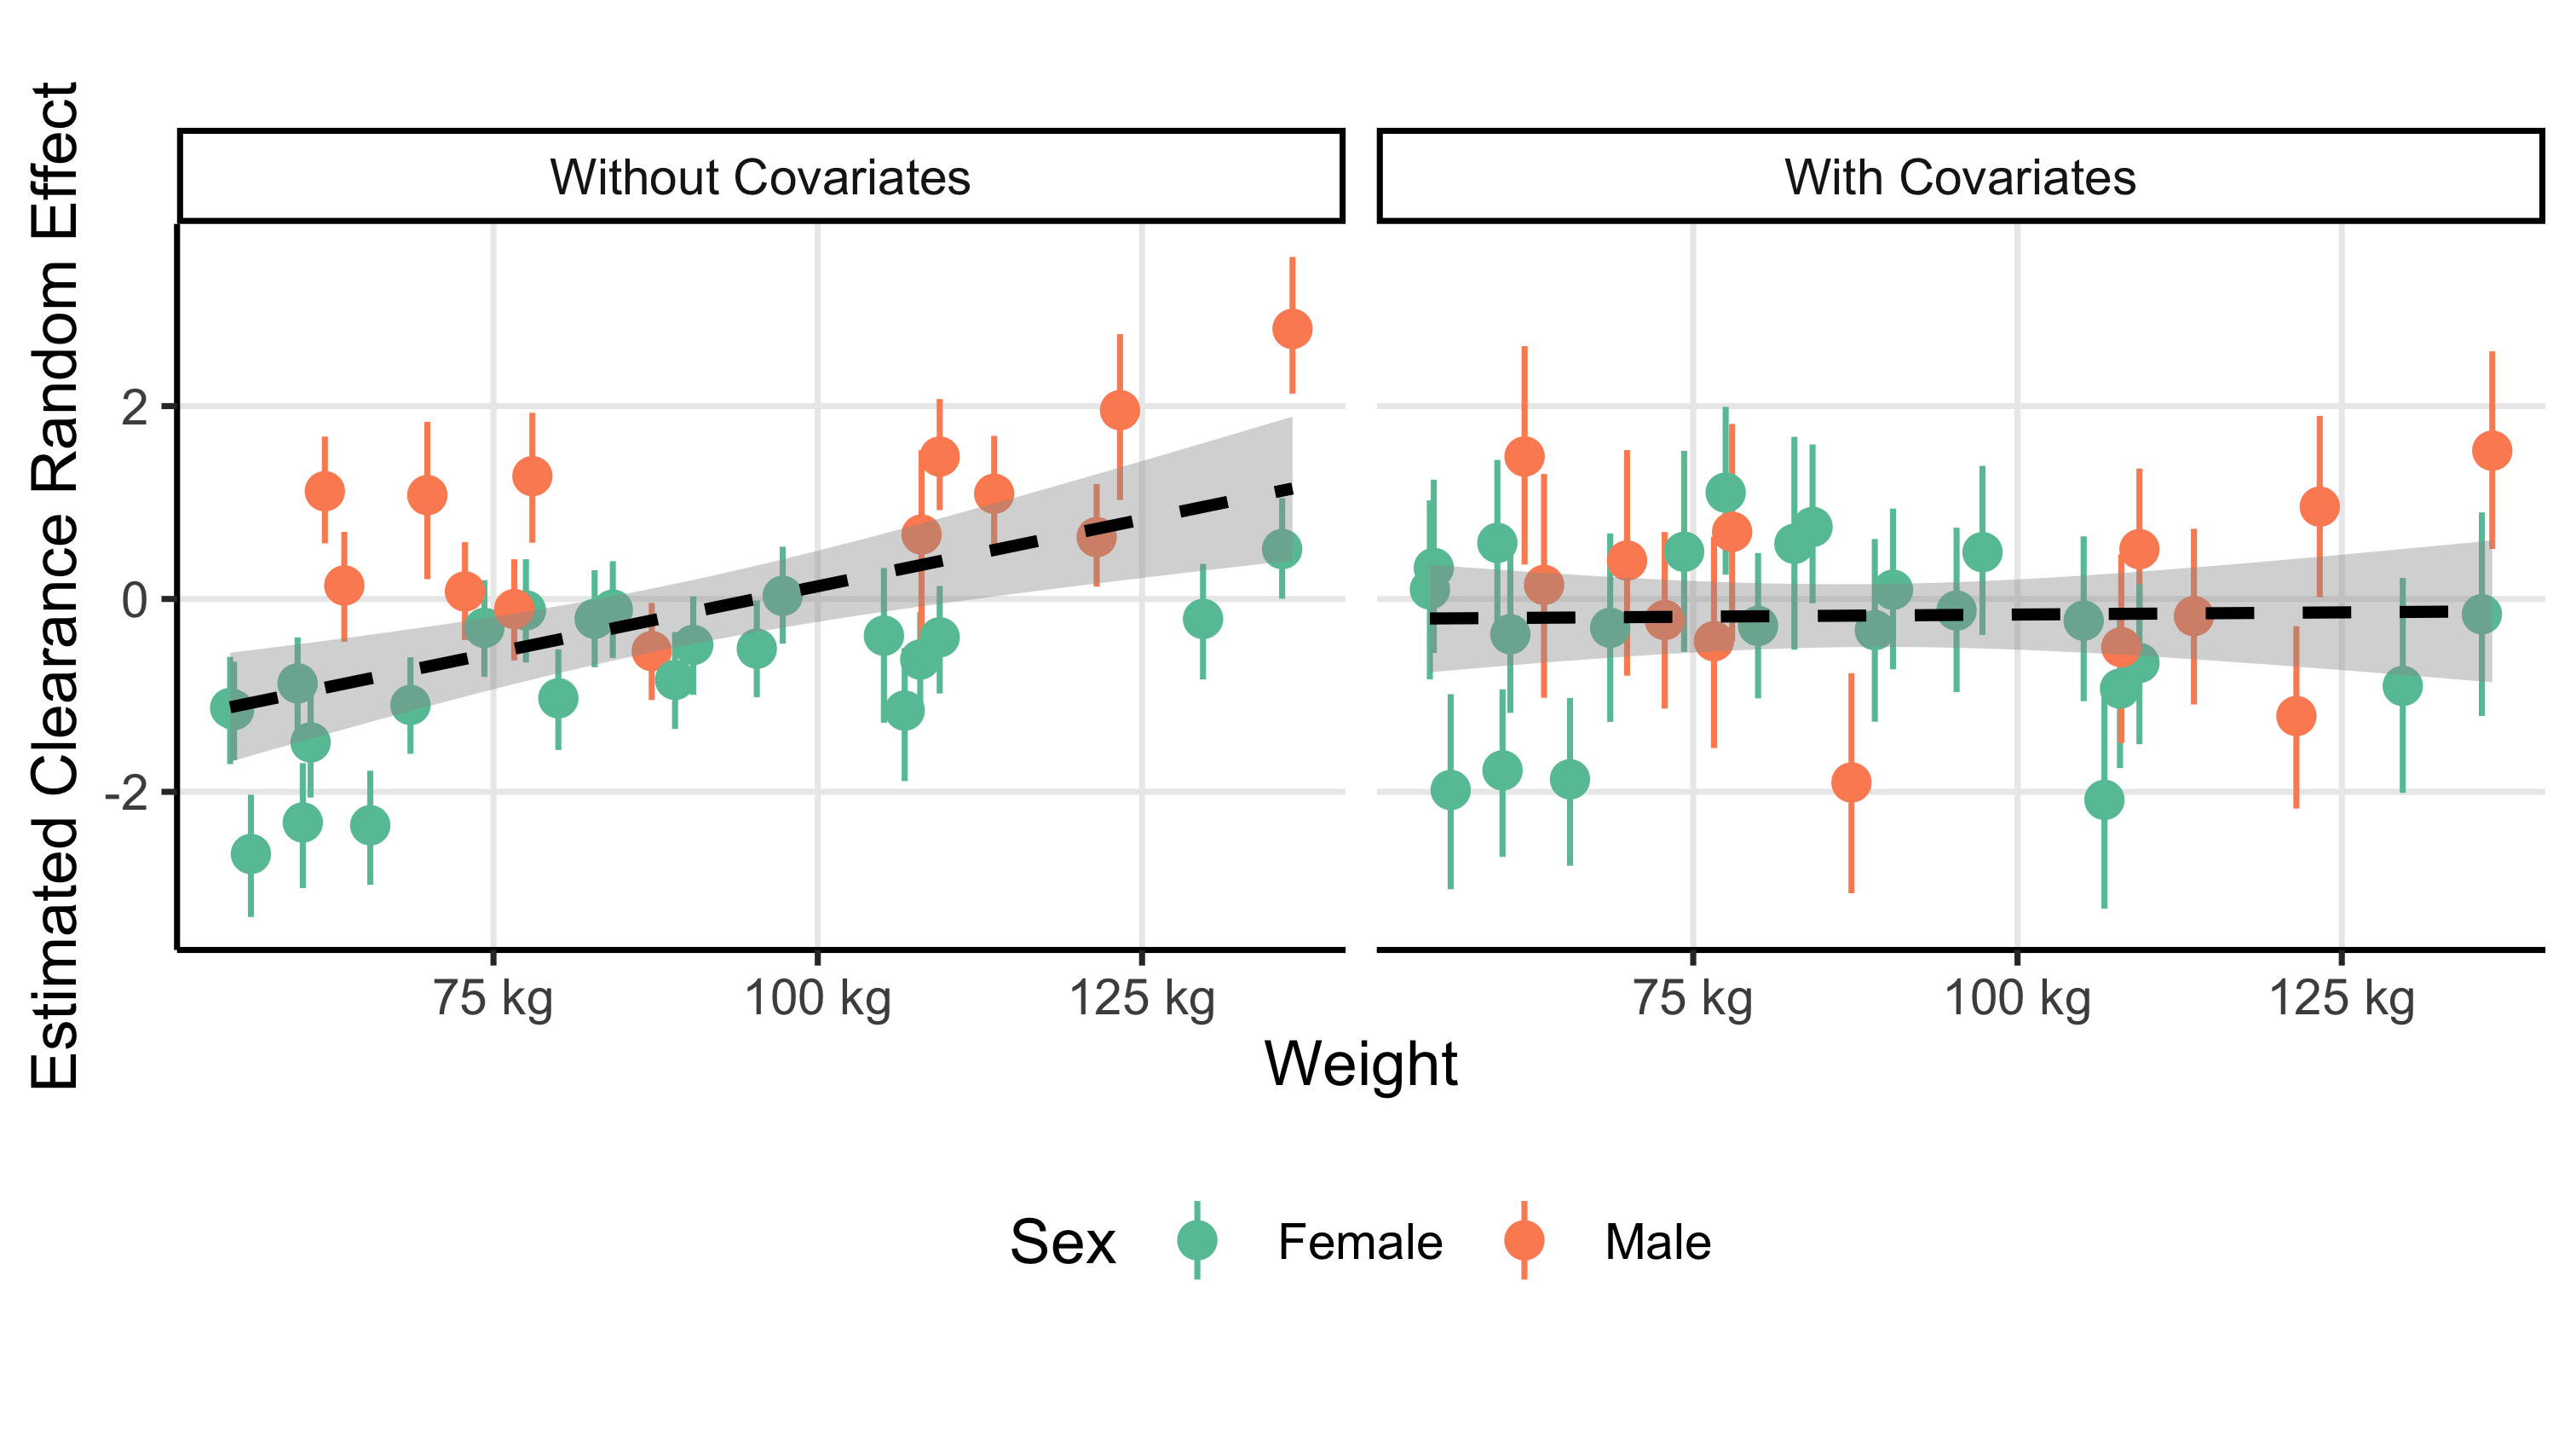
\includegraphics[width=\linewidth]{"figures/random_effects_change.png"}
	\caption{Random effects estimates for clearance $ CL_i $ and 95\% credible intervals (left).  Random effects estimates are colored by patient sex.  Prior to adjusting for covariates, a general trend in weight can be seen in the random effects.  Subjects who are heavier tend to have larger random effect, and males tend to have larger random effects than females of the same weight.  Patterns such as these indicate that weight and sex can be used to explain variation in the random effects.  After adjusting for sex and weight (right), the random effects have no discernable pattern.}
	\label{fig:randomeffectschange}
\end{figure}

We fit our model to real pharmacokinetic data using the open source probabalistic programming language, Stan \cite{gelman2015stan}.  Stan monitors several Markov chain diagnostics, none of which detected problematic Markov chain behavior, which indicates that Stan’s sampling algorithm was able to converge (0 divergences, all all Gelman-Rubin diagnostics<1.01, all effective sample sizes  > 2600).  

The inclusion of covariates in the model results in a better fit than excluding them. Shown in \cref{fig:randomeffectschange} are the estimated random effects for the clearance pharmacokinetic parameter of each subject as a function of weight.  Subject sex is indicated by color, the overall trend is shown in the black dashed line.  Failing to include subject sex and weight results in males having on average a larger random effect than females of the same weight, and heavier subjects having a larger random effect than lighter subjects.  When covariates are added into the model, the variation in the random effects attenuates, resulting in closer alignment to model assumptions. A better fit to the data means data generated from the model may be closer aligned with the true data generating process.

Examining the posterior distributions of the regression coefficients provides further insights into the relationships between covariates and pharmacokinetics. Greater subject weight is associated with an increase in the expected value of alpha (which is used to compute the elimination and absorption rates in the first order one compartment PK model.  The parameter $ \alpha $ is the ratio of how fast the drug exits the central compartment  how fast the drug enters the central compartment) which impacts the time to maximum concentration after each dose.  There is an estimated effect of sex on $ \alpha $ (males have smaller alpha than females, meaning the drug leaves their central compartment slower or enters the central compartment quicker), however the uncertainty is large (estimated effect -0.2 on the logit scale, 95\% credible interval -0.53 to 0.15). See \cref{tab:coefs} in the Appendix for a full summary of the regression coefficients.


%\begin{figure}
%	\centering
%	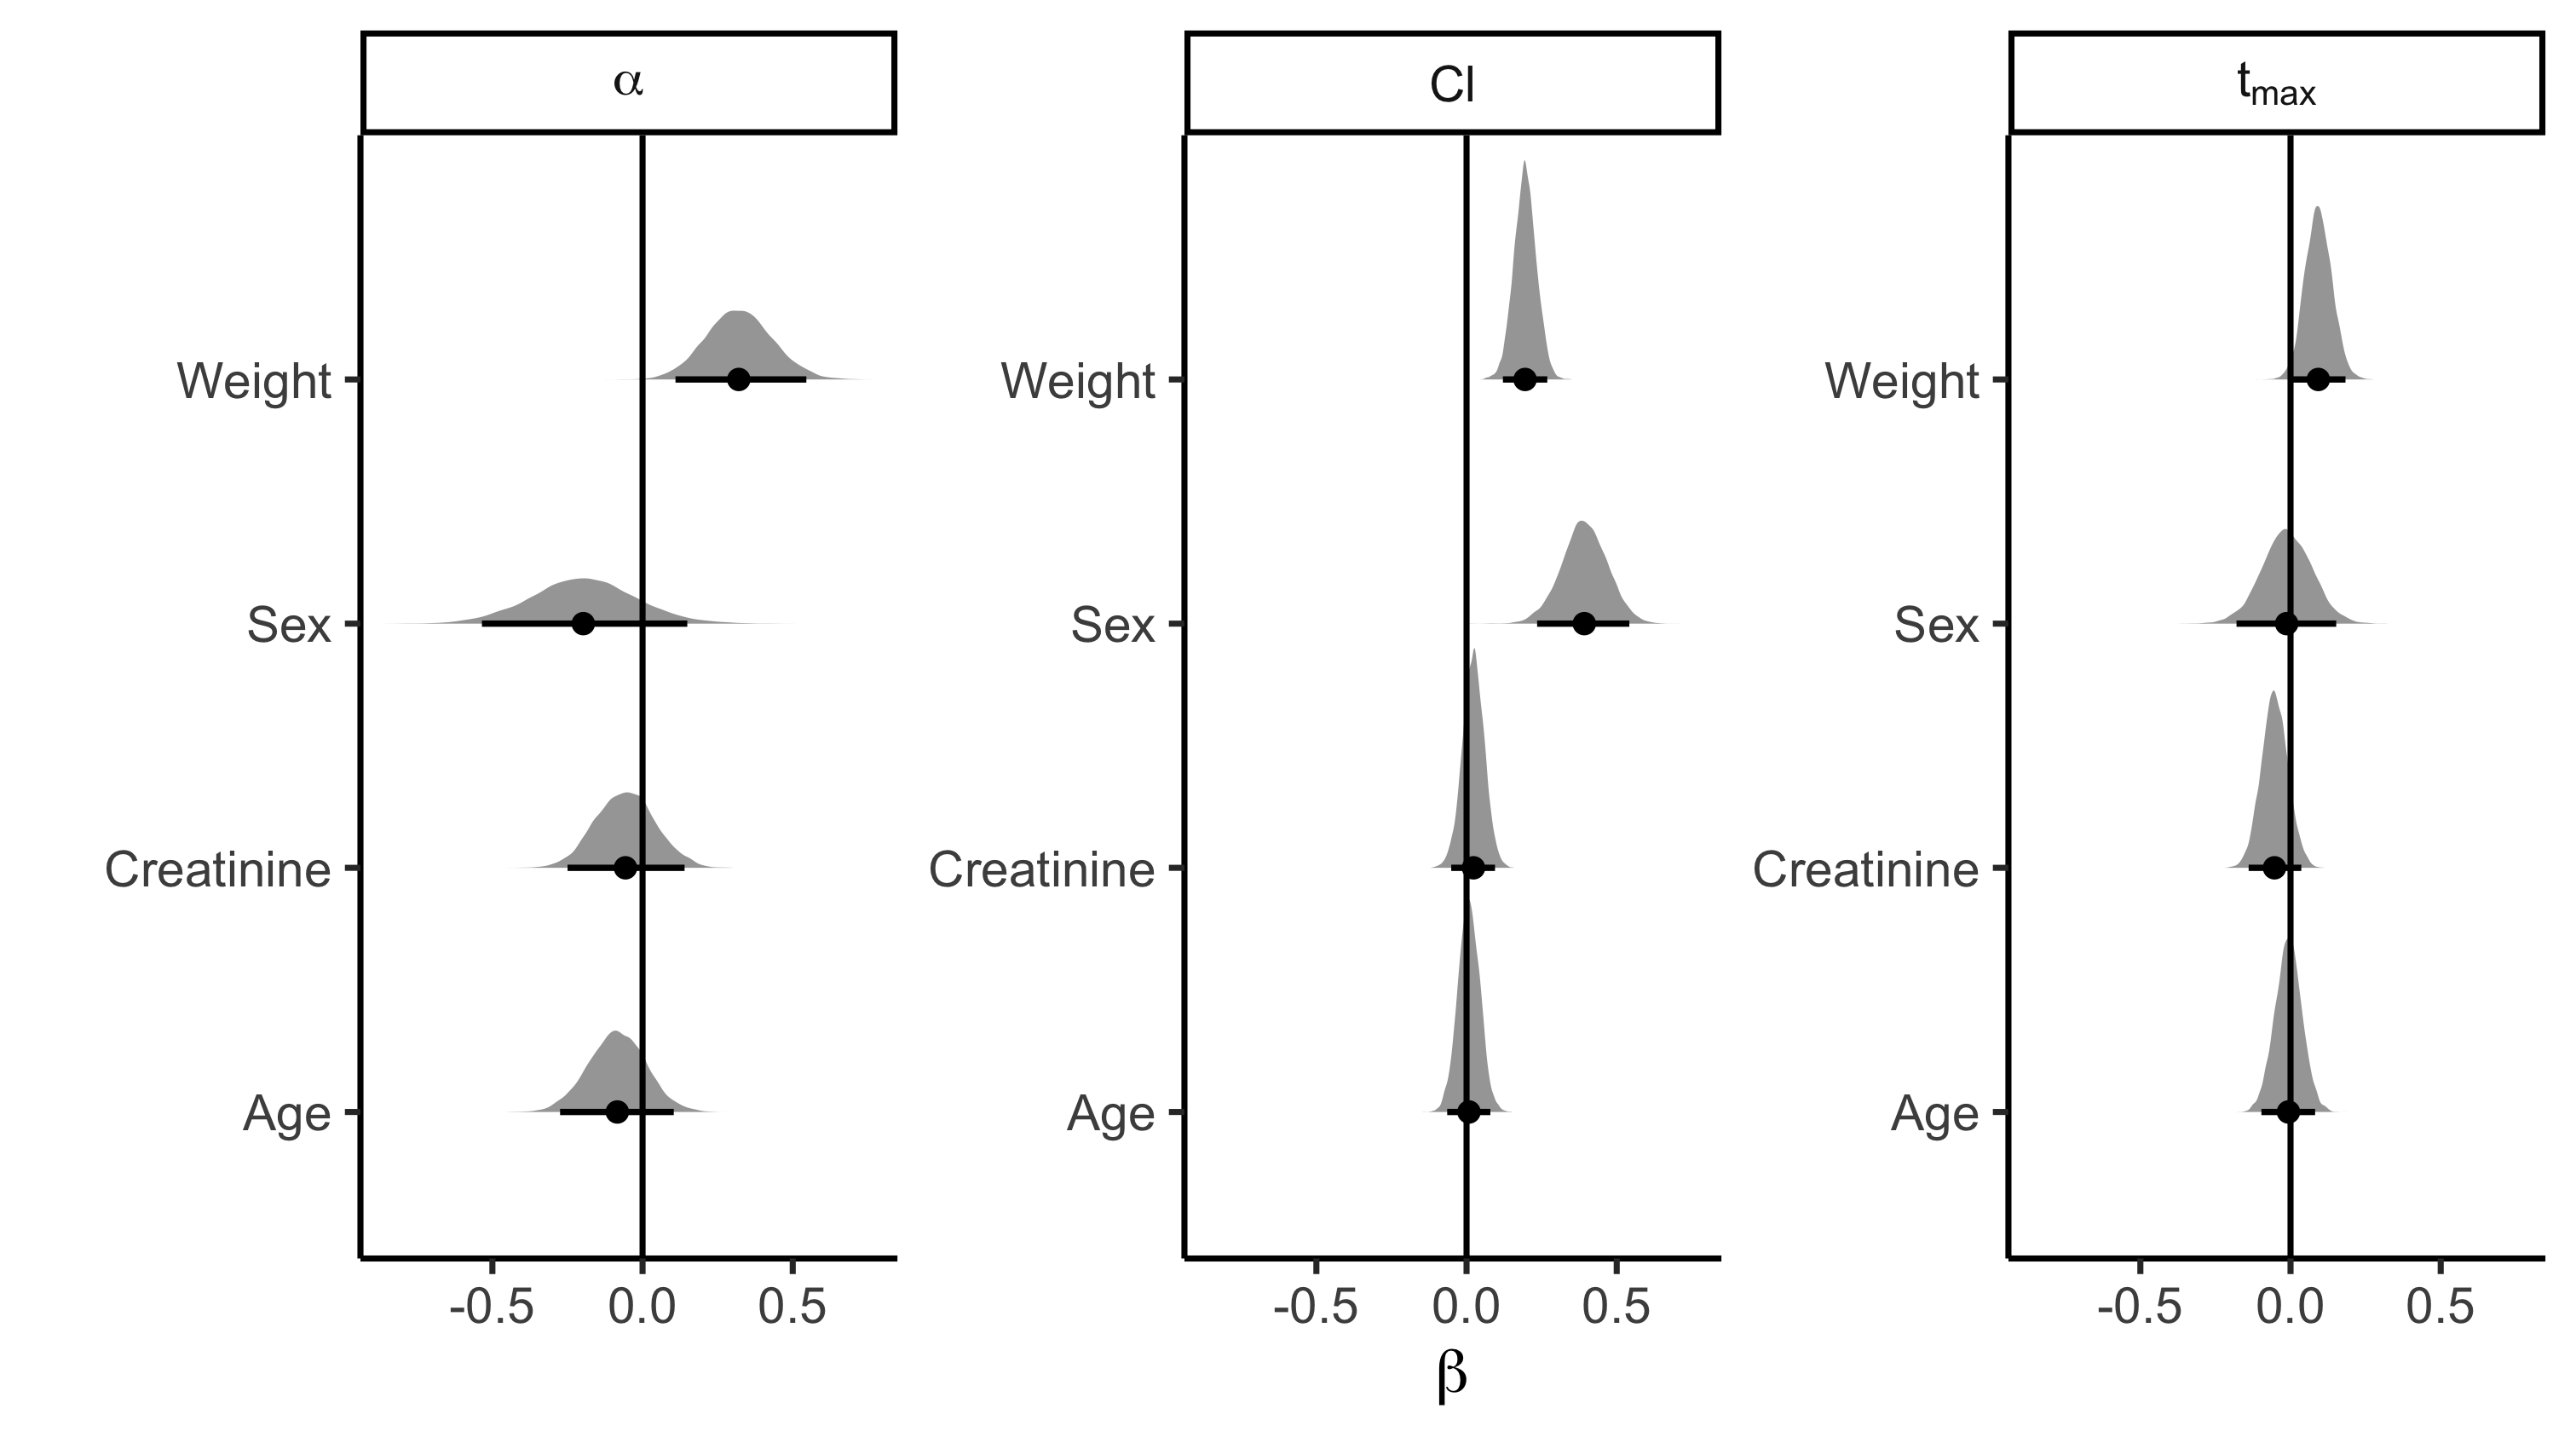
\includegraphics[width=1\linewidth]{figures/coef_vals}
%	\caption{Posterior distributions of regression coefficients. Expectations are shown as black dots, 95\% credible intervals are shown as horizontal black lines.  Solid black vertical line is $\beta=0$ for reference.  Note, regression coefficients for $Cl$ and $t_{max}$ act multiplicatively (a one unit increase in weight leads to a change in $Cl$ of $\exp(\beta)$), while regression coefficients for $\alpha$ are interpreted on the log odds scale.}
%	\label{fig:coefvals}
%\end{figure}


Model training error is comparable between the two models; the model without covariates achieves an average error of 8.31 ng/ml as measured by root mean squared error.  The model with covariates achieves a root mean squared error of 8.36  ng/ml.  Estimates of concentration uncertainty remain similar between the two models as well.  We conclude the inclusion of covariates in the model improves model inferences but does not substantially improve the fit of the model in this case.

While prediction error and concentration uncertainty are comparable between the two models, the most important differences are between inter-individual uncertainty.  The inclusion of the covariates explains variation between individual pharmacokinetic parameters, hence the between subject variability $\sigma_{Cl}, \sigma_{t_{max}}$ and $\sigma_\alpha$ are smaller in the covariate model as opposed to the no covariate model.  This uncertainty effects decision making, as the no covariate model is more uncertain about the pharmacokinetics of new patients.

\end{document}